\documentclass[reprint,amsmath,amssymb,aps,prl,floatfix,groupedaddress,superscriptaddress]{revtex4-2}
\usepackage{graphicx}% Include figure files
\usepackage{comment}
\usepackage[caption=false]{subfig}
\usepackage{dcolumn}% Align table columns on decimal point
\usepackage{bm}% bold math
%\usepackage{hyperref}% add hypertext capabilities
\usepackage[mathlines]{lineno}% Enable numbering of text and display math
\usepackage{mathtools}
\usepackage{physics}
\usepackage{times,newtx}
\usepackage{hyperref}
\usepackage{color}
\usepackage{overpic}
\renewcommand{\bibfont}{\fontsize{8.5pt}{9.5pt}\selectfont}
% \linenumbers\relax % Commence numbering lines



%\usepackage[showframe,%Uncomment any one of the following lines to test
%%scale=0.7, marginratio={1:1, 2:3}, ignoreall,% default settings
%%text={7in,10in},centering,
%%margin=1.5in,
%%total={6.5in,8.75in}, top=1.2in, left=0.9in, includefoot,
%%height=10in,a5paper,hmargin={3cm,0.8in},
%]{geometry}

% \newcommand{\bra}[1]{\langle #1 |}
% \newcommand{\ket}[1]{| #1 \rangle}
% \newcommand{\braket}[2]{\langle #1| #2\rangle}
% \newcommand{\pdv}[2]{\frac{\partial #1}{\partial #2}}
% \newcommand{\Tr}{\text{Tr}}
\renewcommand{\var}[1]{\text{var} (#1) }
\newcommand{\cov}[2]{\text{cov} (#1, #2) }
\DeclarePairedDelimiter\floor{\lfloor}{\rfloor}

\begin{document}

%\preprint{APS/123-QED}

\title{Quantum Limits of Passive Optical Surface Metrology and Defect Detection}% Force line breaks with \\

\author{Jernej Frank}
\email{jernej.frank@physics.ox.ac.uk}
\affiliation{%
 Department of Physics, University of Oxford, Oxford, OX1 3PU, UK
}

\author{George Brumpton}
\email{pmygb8@nottingham.ac.uk}
\affiliation{%
 {Manufacturing~Metrology~Team,~Faculty~of~Engineering,~University~of~Nottingham,~Nottingham~NG7~2RD,~UK}
}%

\author{Tommaso Tufarelli}
\affiliation{%
School of Mathematical Sciences and Centre for the Mathematics and Theoretical Physics of Quantum Non-Equilibrium Systems, University of Nottingham, University Park, Nottingham NG7 2RD, UK}%

\author{Gerardo Adesso}
\email{gerardo.adesso@nottingham.ac.uk}
\affiliation{%
School of Mathematical Sciences and Centre for the Mathematics and Theoretical Physics of Quantum Non-Equilibrium Systems, University of Nottingham, University Park, Nottingham NG7 2RD, UK}%

\author{Samanta Piano}
\email{samanta.piano@nottingham.ac.uk}
\affiliation{%
 {Manufacturing~Metrology~Team,~Faculty~of~Engineering,~University~of~Nottingham,~Nottingham~NG7~2RD,~UK}
}%

\date{\today}% It is always \today, today,
             %  but any date may be explicitly specified

% With abstracts, I typically aim for a 5-sentence model that mirrors the structure of the rest of the paper:
% S1: what we know
% S2: what we don't
% S3: how you answer that question
% S4: what you find
% S5: why it's important
\begin{abstract}
We develop a quantum statistical framework for passive optical surface metrology. Modelling a surface as an incoherent ensemble of point emitters imaged through a diffraction-limited system, we employ techniques from quantum parameter estimation and hypothesis testing to derive ultimate bounds for jointly estimating geometrical features and for deciding the presence or absence of surface defects, and we identify optimal measurements from the geometry of the point-spread-function manifold.  As a representative application, we analyse a minimal surface crack model based on three point sources and show that spatial mode sorting can simultaneously enable near-quantum-limited estimation of crack width and depth and markedly enhanced detectability of the crack, compared with direct imaging. Our results pave the way towards enhanced optical inspection and characterisation of sub-diffraction surface features by probing a limited number of spatial modes without any illumination control.
\end{abstract}
%Optical surface metrology comprises many techniques for estimating surface parameters. It offers a faster alternative over mechanical profilometry, with decreased accuracy due to the diffraction nature of optics and reliance on mathematical reconstruction models instead of measuring the surface directly.
%Our investigation into the precision bounds of optical methods has led us to propose novel measuring schemes that have the potential to revolutionise accuracy in optical surface metrology. By generalising the analysis of quantum and classical Fisher information from two-point source problems to an arbitrary number of point sources, we propose a discrete imaging model for its real-world continuous counterpart.
%We find that passive measurement schemes can improve accuracy in estimating descriptive parameters for surface defects. Our analysis opens the possibility that estimation parameters have a corresponding measurement basis vector that contributes most of the information necessary to estimate it. Lastly, the insights lead to improved measurement schemes in optical metrology and pave the way towards a general imaging description using parameter estimation approaches.



\maketitle


\paragraph{\bfseries Introduction.\label{sec:intro}}
Optical surface metrology enables non-contact measurement of three-dimensional (3D) surface topography using light \cite{leach2020advances,catalucci2022optical}. Compared with contact-based techniques, optical approaches can enable faster and less invasive measurements over extended surface areas \cite{hocken2005optical}. In practice, optical surface metrology encompasses a range of techniques that may rely on controlled illumination ({\em active} methods), such as structured-light or interferometric profilometry \cite{yang2022single,van2019deep,wang2021single,li2016single}, or instead exploit naturally available or uncontrolled illumination ({\em passive} methods) \cite{mathia2011recent,marrugo2020state}. In both cases, the achievable precision is ultimately limited by diffraction and by the information that can be extracted from the detected optical field.


In this Letter, we analyse optical surface metrology from the perspective of {\em quantum} parameter estimation and hypothesis testing, to formulate the ultimate precision bounds and propose measurements approaching them. This line of inquiry originates from Tsang's seminal work \cite{tsang2016quantum}, which demonstrated that quantum measurements can overcome classical resolution limits in estimating the separation between two sources.
%Rather than relying on spectral decompositions of the density matrix,  we
Adopting a non-orthogonal basis formulation \cite{fiderer2021general,napoli2019towards,genoni2019non}, our study reveals that the quantum limits are governed entirely by pairwise overlaps of the  point-spread functions (PSFs) and by the tangent directions generated by infinitesimal displacements. This structure directly identifies physically meaningful measurement modes tailored to specific surface parameters.


We illustrate our framework on the technologically relevant task of {\em estimating the depth and width of a surface crack}. We focus on a minimal model in which the crack profile is represented by three point sources, allowing a complete quantitative analysis based on Fisher information. We additionally address the complementary problem of {\em crack detection}, formulating it as a binary hypothesis test \cite{GG} and deriving analytical and numerical bounds on the Chernoff information governing the discrimination performance. In both estimation and detection settings, we compare classical direct imaging with experimentally accessible {\em spatial mode sorting} \cite{modes,starlight,da2021super,MPLC,Paur:16,Yang:16,Tham:17,zhou2019quantum,Zanfo,Frank:23,bradypo}. We show that the latter enables substantial precision gains, reaching the ultimate quantum limits using purely passive optical measurements. {\color{red} In contrast to previous applications of quantum metrology to 3D discrete imaging~\cite{fiderer2021general,napoli2019towards}, this work treats the joint estimation of crack width and depth from the geometry of the PSF manifold. The closed-form quantum Fisher information matrix is expressed entirely through PSF overlaps, which directly identifies the optimal measurement modes. We derive closed form solutions for MS measurements for arbitrary polynomial bases that allow us to investigate convergence of the Cram\'er-Rao bound to the quantum Cram\'er-Rao bound under realistic experimental conditions.}


\paragraph{\bfseries Preliminaries.\label{sec:prelim}}
We recall the quantum statistical tools that will be used to derive error bounds for surface characterisation.

\paragraph{Parameter estimation theory.\label{sec:parameterestimation}}
We consider $m$ distinct parameters $\theta = (\theta_1,\theta_2,\dots,\theta_m)$ for which we aim to build estimators $ \hat{\theta} = (\hat{\theta}_1,\hat{\theta}_2,\dots,\hat{\theta}_m)$. For any unbiased estimation strategy specified by a measurement $\Pi$, the error covariance matrix $\text{cov}(\theta)$ is lower bounded by the classical Cram\'er-Rao bound \cite{lehmann2006theory,van2004detection}, which in turn is lower bounded by the quantum Cram\'er-Rao bound \cite{helstrom1969quantum,braunstein1994statistical}
\begin{align}
    \text{cov}(\theta) &\geq N^{-1} J_\Pi^{-1} \geq N^{-1} H^{-1},
\end{align}
with $N$ being the number of measurements, $J_\Pi$ the Fisher information matrix (FIM) and $H$ the quantum Fisher information matrix (QFIM). The inequalities mean that $N\text{cov}(\theta) - J_\Pi^{-1}$  and $H-J_\Pi$ are positive semidefinite matrices for all $\Pi$. If we implicitly define the symmetric logarithmic derivative (SLD) $\Lambda_a$ related to the parameter $\theta_a$ ($a=1,\dots,m$) as
\begin{align}
   2{\partial_{\theta_a} \rho} = \rho \Lambda_a+ \Lambda_a \rho,
\label{def:sld}
\end{align}
for a parameter-dependent density operator $\rho=\rho(\theta)$, we can express the QFIM matrix elements as
\begin{align}
    H_{a,b} = \text{Tr} \left [ \Lambda_{a} {\partial_{\theta_b} \rho} \right ].
\label{def:QFIM}
\end{align}
Assuming Poissonian counting statistics \cite{tsang2018subdiffraction} to account for typical optical photon losses, the FIM can be written as
\begin{align}
    ({J_\Pi})_{a,b} &= \tau \sum_j^M\frac{1}{P_j(\theta)} \pdv{P_j(\theta)}{\theta_a}  \pdv{P_j(\theta)}{\theta_b},
\label{eq:FI_MS}
\end{align}
where $P_j(\theta) = \int dr\, \big|\!\braket{\phi_j}{\psi}\!\big|^2 F(r|\theta)$ is the mean detected power in a measurement channel $\phi_j$ for an object distribution $F(r|\theta)$, with $\ket{\psi}$ the PSF of the optical system, $\tau$ the Poissonian detection rate, and $M$ the number of measurement channels.

If we are interested in estimating a different set of parameters, say $\Tilde{\theta}$, which can be expressed as functions of the original parameters $\theta$, then the corresponding QFIM and FIM are transformed via the Jacobian of the re-parametrisation \cite{paris2009quantum,liu2020quantum},
\begin{align}
    \Tilde{H} &= B H B^\top, \quad
    B_{\alpha,b} = \partial{\theta_b}/\partial{\Tilde{\theta}_\alpha}, \quad     \Tilde{J_\Pi} = B J_\Pi B^\top.
    \label{def:jacobian}
\end{align}

%\paragraph{Non-orthogonal basis approach.}
To preserve the physical and geometric picture of the underlying problem, we will use a non-orthogonal basis to calculate the QFIM \cite{genoni2019non,napoli2019towards,fiderer2021general}. Given a (generally non-orthogonal) basis $\{\ket{\psi_v}\}, v = 1,2,\dots$, which spans the subspace relevant to the estimation problem, we can then expand all operators of interest as:
$\rho = \sum_{u,v} R^{u,v} \ket{\psi_u}\bra{\psi_v}$, $\pdv{\rho}{\theta_a} = \sum_{u,v} D_a^{u,v} \ket{\psi_u}\bra{\psi_v}$,
$\Lambda_a =  \sum_{u,v} L_a^{u,v} \ket{\psi_u}\bra{\psi_v}$,
which implicitly define the matrices ${R}, D_a$ and $L_a$. Then, the $a^{\textrm{th}}$ SLD in Eq.~\eqref{def:sld} becomes
\begin{align}
    2 {D}_a = {L}_a{G}{R} + {R}{G}{L}_a,
    \label{eq:sld_nonorthogonal}
\end{align}
and the QFIM Eq.~\eqref{def:QFIM} transforms into
\begin{align}
    H_{a,b} = \Re \Tr (L_a G D_b G) =  \Re \Tr( R G L_a  G L_b G),
    \label{eq:qfi_nonorthogonal}
\end{align}
where we define the Gram matrix $G_{u,v}=\braket{\psi_u}{\psi_v}$ to account for the potential non-orthogonal basis representation.
%In case the basis is orthogonal the Gram is the identity matrix and we recover the previous expression.

\paragraph{Quantum hypothesis testing.\label{sec:hypothesistesting}}
We consider a binary quantum hypothesis test to discriminate between two states $\rho_0$ (null hypothesis) and $\rho_1$ (alternative hypothesis). For a  measurement $\Pi$, a decision rule can yield a type I error (false positive) with probability $\alpha$ and a type II error (false negative) with probability $\beta$. In the asymptotic limit of $N \gg 1$ identical runs, the symmetric error probability  $P_{\textrm{err}} = (\alpha + \beta)/2$ decreases exponentially as $P_{\textrm{err}}(N) \sim e^{-N \xi_{\Pi}}$. The asymptotic error exponent $\xi_{\Pi}$, which quantifies the distinguishability between the two hypotheses, is given by the Chernoff information \cite{cover1999elements},
\begin{equation} \label{eq:CCB}
    \xi_{\Pi} = - \min_{0 \leq s \leq 1} \log \Big( \sum_x P_0(x)^s P_1(x)^{1-s} \Big),
\end{equation}
with $P_j$ the outcome probability distribution for $\rho_j$ ($j=0,1$). Maximizing $\xi_{\Pi}$ over all possible measurements yields the quantum Chernoff bound (QCB) $\xi_Q \geq \xi_\Pi$, which represents the ultimate upper limit on asymptotic distinguishability and can be evaluated directly from the density matrices \cite{audenaert2007discriminating},
\begin{equation} \label{eq:QCB}
\xi_Q = - \min_{0 \leq s \leq 1} \log \text{Tr} \big[ \rho_0^s \rho_1^{1-s} \big].
\end{equation}


\paragraph{\bfseries Quantum precision bounds for discrete imaging models.\label{sec:CR-bounds} }
Assuming no \textit{a priori} control  over the illumination, we model a surface as a discrete grid of points in 3D space, each emitting photons that get collected by a lens. For monochromatic light of wavelength $\lambda$ and a circular aperture, the spatial probability distribution of photons from a single point source in the image plane defines the PSF, described by a Gaussian beam
\begin{equation}
\begin{aligned}
\label{def:psf}
\!\!    &\psi_v (x+\delta x_v,y+\delta y_v,z+\delta z_v) = \sqrt{\frac{1}{\pi}} \frac{i}{z+\delta z_v + i} \\
\!\!    &\times \exp{\frac{-i((x+\delta x_v)^2 + (y+ \delta y_v)^2)}{2(z+\delta z_v + i)} - ikz_R(z+\delta z_v)},
\end{aligned}
\end{equation}
where $(x,y,z)$ are the coordinates in the object plane, $(\delta x_v,\delta y_v,\delta z_v)$ are displacements of the point source $v$ from the origin in the object plane, $k= 2\pi / \lambda$ is the wave vector and $z_R$ the Rayleigh length. We renormalised the coordinate system to use relative length scales, $x \rightarrow \sqrt{k/z_R}x$ and $ z \rightarrow z/z_R$.

In the weak-source regime \cite{tsang2016quantum}, we can represent an object consisting of $V$ incoherent point sources by the mixed state
\begin{align} \label{eq:incoherent_ensemble}
    R = {\sum}_v^V I_v \ket{\psi_v}\bra{\psi_v},
\end{align}
where $\ket{\psi_v} = \int \psi_v (x+\delta x_v,y+\delta y_v,z+\delta z_v) \ket{xyz}$ is the PSF centered at the displaced point source $(\delta x_v,\delta y_v,\delta z_v)$ from the origin and $I_v$ its relative intensity, with $\sum_v I_v=1$.

The states ${\ket{\psi_v}}$ are non-orthogonal: their mutual overlaps encode the diffraction-induced indistinguishability between nearby surface features. %Computing the QFIM to find the ultimate precision bounds can therefore be viewed as evaluating the maximal quantum statistical metric on the PSF manifold embedded in Hilbert space.
The relevant information about the displacement parameters $\theta = (\theta_v^a) \equiv (\delta x_v,\delta y_v,\delta z_v)$ is contained in the tangent directions generated by infinitesimal shifts of each PSF. %\textcolor{blue}{
Since in general $\ket{\partial_{\theta_u^a}\psi_u}$ is linearly independent from the states $\ket{\psi_v}$,%},
%these derivative vectors do not lie within the span of ${\ket{\psi_v}}$ alone. We
we must  enlarge the support of the Hilbert space to include the tangent subspace spanned by ${\ket{\partial_{\theta_v^a}\psi_v}}$. This extends the representation from dimension $V$ to $V+3V$.
%, corresponding to the PSF manifold and its associated tangent directions.
In the following, we will assume all point sources have equal intensity $I_v=1/V$ \cite{noteintensity}, leading to a  $3V \times 3V$ QFIM encoding precision bounds for estimating only the  displacements $\theta_v^a$ for each point source $v=1,\ldots,V$ {\color{red}(unequal intensities only reallocate Fisher information between the crack width and depth under a fixed photon budget; see Appendix~\ref{app:unequal_intensities})}.

Ordering the basis vectors as $\big\{|{\psi}\rangle$, $|{\partial_{\delta x_v} \psi}\rangle$, $|{\partial_{\delta y_v} \psi}\rangle$, $|{\partial_{\delta z_v} \psi}\rangle\big\}$, we write all matrices in block matrix form
\begin{align}\label{eatlean}
    X &= \begin{pmatrix}
        X_\Delta & X_\gamma\\
        X_{\gamma^\dagger} & X_\tau
    \end{pmatrix},
\end{align}
where $X_\Delta \in V \times V$ represents the PSF manifold geometry, $X_\tau \in 3V \times 3V$ the curvature structure (overlaps between tangent vectors), and $X_\gamma \in 3V \times V$ and its adjoint $X_{\gamma^\dagger}$ the first-order sensitivity (PSF–tangent couplings).
Assuming Gaussian beams Eq.~\eqref{def:psf}, the Gram matrix $G$ can be evaluated analytically (see Appendix~\ref{app:gaussian_overlaps} \cite{supposta}),
while the density matrix has support only on the first block $\Delta$, $R_\Delta = \frac{1}{V} \openone_V$,
with $\openone_V$ the $V\times V$ identity matrix, and each derivative matrix becomes sparse with only two non-zero entries,
    $D_a^{\partial u,u} = D_a^{u,\partial u} = \frac{1}{V}$ (where the $\partial u$ superscript corresponds to the basis vector $\ket{\partial_{\theta_u^a} \psi_u}$).
Solving for the QFIM Eq.~\eqref{eq:qfi_nonorthogonal} in this basis results in the closed-form solution (see Appendix~\ref{app:qfi_derivation} \cite{supposta})
\begin{align}
    H_{a,b} &= 2 \Re \langle{\gamma^b}| G_{\gamma^\dagger} L^a_\Delta G_\Delta |{\gamma^b}\rangle \nonumber\\
    &+ 4 \Re \langle{\gamma^a}|G_{\gamma^\dagger}|{\gamma^b}\rangle\langle{\gamma^b}|G_{\gamma^\dagger} G^{-1}_\Delta|{\gamma^a}\rangle,
    \label{eq:qfim_final}
\end{align}
where $G^{-1}_\Delta$ is the inverse PSF overlap matrix, $\ket{\gamma^a}$ (resp. $\ket{\gamma^b}$) are the basis vectors encoding derivative matrices $D_{\gamma^{a}}$ (resp. $D_{\gamma^{b}}$), and $L^a_\Delta$ is defined by the reduced Lyapunov equation
\begin{align}
    L^a_{\Delta} G_{\Delta} + G_{\Delta} L^a_{\Delta}  &= -2 (G_{\gamma}D_{\gamma^{a\dagger}}G_\Delta^{-1} + G_\Delta^{-1} D_{\gamma^a}G_{\gamma^\dagger}).
    \label{eq:L_delta_sylvester}
\end{align}
Since $G_\Delta$ is Hermitian and invertible, each $L_\Delta$ is unique and the corresponding SLD operators are Hermitian. The final expression for the QFIM Eq.~\eqref{eq:qfim_final} shows that the quantum Fisher information depends solely on the PSF overlap matrix $G_\Delta$ and its couplings to first-order derivatives  $G_{\gamma} $ (resp. $G_{\gamma^\dagger}$). %No spectral decomposition of the density operator is required.
The ultimate precision bounds are therefore determined entirely by the local overlap geometry of the PSF manifold. For a Gaussian PSF, the derivative directions are proportional to Hermite-Gaussian functions of increasing order, which motivates the study of spatial mode sorting in the Hermite polynomial basis \cite{weisstein2002hermite} as an optimal measurement strategy \cite{starlight,rehacek2017optimal}.


\begin{figure}[t]
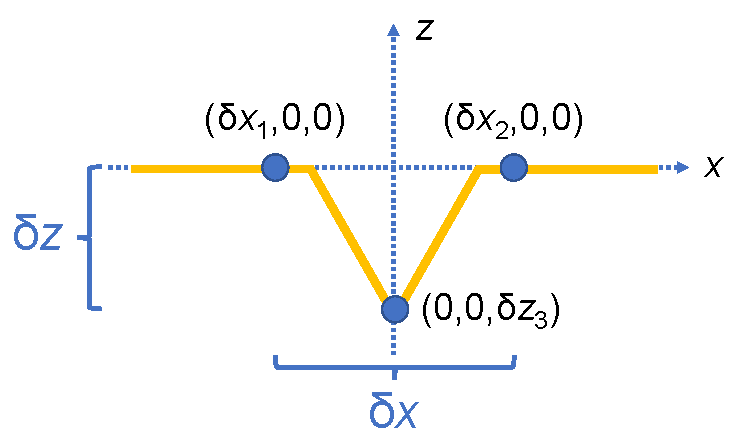
\includegraphics[width=.6\columnwidth]{model_three.pdf} \vspace*{-0.25cm}
\caption{\label{fig:3source_layout}Representation of a surface crack with width parameter $\delta x$ and depth parameter $\delta z$, modelled by three incoherent point sources.}
\end{figure}

\paragraph{\bfseries Application: Surface crack inspection.\label{sec:3src}}
We now apply our general methods to the concrete problem of analysing {\em surface cracks}. We will explore two tasks: (i) estimating geometric parameters of a crack, via Fisher information, and (ii) detecting the presence of a crack, via Chernoff information.

In our toy model, a crack is described by three point sources placed symmetrically on the $x$-axis, with the third (middle) one displaced along the $z$-axis [Fig.~\ref{fig:3source_layout}]. We relate the coordinates of the point sources to two parameters that characterise the problem, i.e., the width $\delta x$ and depth $\delta z$ of the crack,
\begin{equation}
\begin{aligned}
    \delta x &\coloneqq {\delta x_2 - \delta x_1}, \quad     \delta z \coloneqq -\delta z_3.\
\end{aligned}
\label{eq:3pt2paramcoords}
\end{equation}

\paragraph{(i) Estimating width and depth of the crack.}
The ultimate precision bound on estimating individual source displacements (${\delta x_1},{\delta x_2},{\delta z_3}$) is given by the QFIM from Eq.~(\ref{eq:qfim_final}). We collapse the QFIM to a $2 \times 2$ matrix for the parameters of interest $\delta x$ and $\delta z$  using Eq.~(\ref{def:jacobian}) with the Jacobian matrix $B = \left(\begin{smallmatrix}
    -\frac{1}{2} & \frac{1}{2} &  0\\
    0 &  0 & -1
    \end{smallmatrix}\right)$.

We now compare two measurement strategies against the quantum precision bound, namely quantum-inspired mode sorting (MS) in the Hermite polynomial basis and the classical direct imaging (DI) approach most commonly utilised. For the MS basis we match the Hermite-Gaussian modes to the PSF, $\phi_{j,l}(x,y) = \frac{H_j(x)}{\sqrt{2^j j!}} \frac{H_l(y)}{\sqrt{2^l l!}} \sqrt{\frac{1}{\pi}} \exp{-\frac{(x^2 + y^2)}{2}}$ and compute the FIM via Eq.~\eqref{eq:FI_MS} using measurement channel probabilities
\begin{align}
    P_{j,l}(\theta) &= \frac{1}{V} \sum_v^V  \abs{ \braket{\phi_{j,l}}{\psi_v(x + \delta x_v, y + \delta y_v, \delta z_v)} }^2 \label{eq:prob_ms_general}
\end{align}
with closed-form expressions provided in Appendix~\ref{app:ms_incoherent} \cite{supposta}.

{\color{red}Guided by the quantum Fisher information, we resolve only the four information-bearing modes $(0,0)$, $(1,0)$, $(2,0)$, $(0,2)$, supplemented by a remainder channel that collects all unresolved light with probability $1-\sum_{(j,l)}P_{j,l}$. This completes the measurement to a valid POVM that registers every photon in the image plane and models the dump port of a realistic mode sorter (Appendix~\ref{app:remainder}).}

For DI, the measurement distribution in the image plane is a sum of the individual intensities $P(x,y|\delta x,\delta z)=\frac13\left[{|{\psi_1(x\!-\!\frac{\delta x}{2},y,0)}|^2\!\! + \!|{\psi_2(x\!+\!\frac{\delta x}{2},y,0)}|^2\!\! + \!|{\psi_3(x,y,-\delta z)}|^2}\right]$, which we integrate numerically to obtain the classical FIM.

We find (see Fig.~\ref{fig:supp4figs} in \cite{supposta}) that the Fisher information confirms the geometric intuition from the QFIM. For estimating the crack width in the sub-Rayleigh regime ($\delta x \rightarrow 0$), the information concentrates  in the $(1,0)$ Hermite-Gaussian mode, corresponding to the first-order transverse PSF derivative. At larger separations, the information spreads across higher-order modes limiting the achievable precision, while  DI approaches the quantum limit instead. Similarly, for depth estimation  ($\delta z\rightarrow0$), MS approaches the quantum limit with equal dominant contributions from the $(2,0)$ and $(0,2)$ modes, which are proportional to second-order transverse PSF derivatives  and span the tangent directions associated with axial defocus{\color{red}, i.e.\ the quadratic wavefront curvature produced by an axial displacement of the point source}. In contrast, the DI Fisher information peaks at the Rayleigh length, consistent with classical beam propagation. {\color{red}The remainder channel still registers the aggregate power of these unresolved modes, recovering part of this information at larger separations (Appendix~\ref{app:remainder}).}

To obtain the Cram\'er-Rao bounds we need to invert the multiparameter FIM. For finite $\delta x$ and $\delta z$, the off-diagonal elements of the FIM are non-zero, showing that width and depth are statistically correlated under generic measurements \cite{ragy2016compatibility}. Nevertheless, measuring in the Hermite-Gaussian mode basis shows the Cram\'er-Rao bound approaching the quantum limit for both $\delta x$ [Fig.~\ref{figshers}(a)] and $\delta z$ [Fig.~\ref{figshers}(b)]. This shows that simultaneous sub-Rayleigh estimation of the crack width and depth is possible using appropriate quantum-inspired measurements. {\color{red}This near-quantum-limited performance is reached with only four resolved modes plus the remainder channel; the leaked fraction is $O(\delta^4)$ in the sub-Rayleigh regime, and resolving further modes helps only beyond the Rayleigh length, where direct imaging is already preferable (Appendix~\ref{app:remainder}).}


% We find (see End Matter, Fig.~\ref{fig:supp4figs}) that the Fisher information for estimating the width $\delta x$ using Hermite MS approaches the quantum limit for small $\delta x$ (with the $(1,0)$ Hermite-Gaussian mode providing the dominant contribution), while it decreases at larger separations due to the finite number of measured modes. In this regime, DI approaches the quantum limit instead. Similarly, for estimating the depth $\delta z$, the Hermite MS Fisher information approaches the quantum limit for small $\delta z$ (with equal dominant contributions from the $(2,0)$ and $(0,2)$ modes due to transverse symmetry). In contrast, the Fisher information for DI is maximised at the Rayleigh length, consistent with classical beam propagation.

% Decomposing the FIM on a per channel contribution shows that in the limits $\delta z \to 0$ and $\delta x \to 0$ we recover the known single-parameter bounds for estimating $\delta x$ \cite{tsang2016quantum} and $\delta z$ \cite{zhou2019quantum}, respectively. Each parameter has a dominating contribution from a single Hermite order: first-order for width estimation and second-order for depth estimation, confirming the geometric picture obtained from the QFIM. Higher-order modes extend the useful parameter range but do not substantially improve precision in the sub-Rayleigh regime.

% As we are estimating both parameters at the same time, we need to invert the FIM to get the Cram\'er-Rao bound. Since the off-diagonal elements for finite $\delta x$ and $\delta z$ are non-zero, the two parameters are not statistically independent [TODO]. For MS measuring in the Hermite basis, the resulting  Cram\'er-Rao bound approaches the quantum Cram\'er-Rao bound for both $\delta x$ [Fig.~\ref{fig:incoh_COV_s}] and $\delta z$ [Fig.~\ref{fig:incoh_COV_p}]. This shows that simultaneous sub-Rayleigh estimation of the crack width and depth is achievable with finite error using an appropriate quantum-inspired measurement basis, outperforming classical DI.


\begin{figure}
\centering
\begin{overpic}[height=4cm]{s_param_covariance_optimal_remainder.pdf}
    % \put(x, y) uses percentages of the image dimensions by default (0-100)
    \put(1, 2){{(a)}}
\end{overpic} \\
\vspace{0.2cm} % Optional: tweak this if you want a tiny gap between top and bottom images
\begin{overpic}[height=4cm]{p_param_covariance_optimal_remainder.pdf}
    \put(1, 2){{(b)}}
\end{overpic}
%\subfloat[]{\label{fig:incoh_COV_s}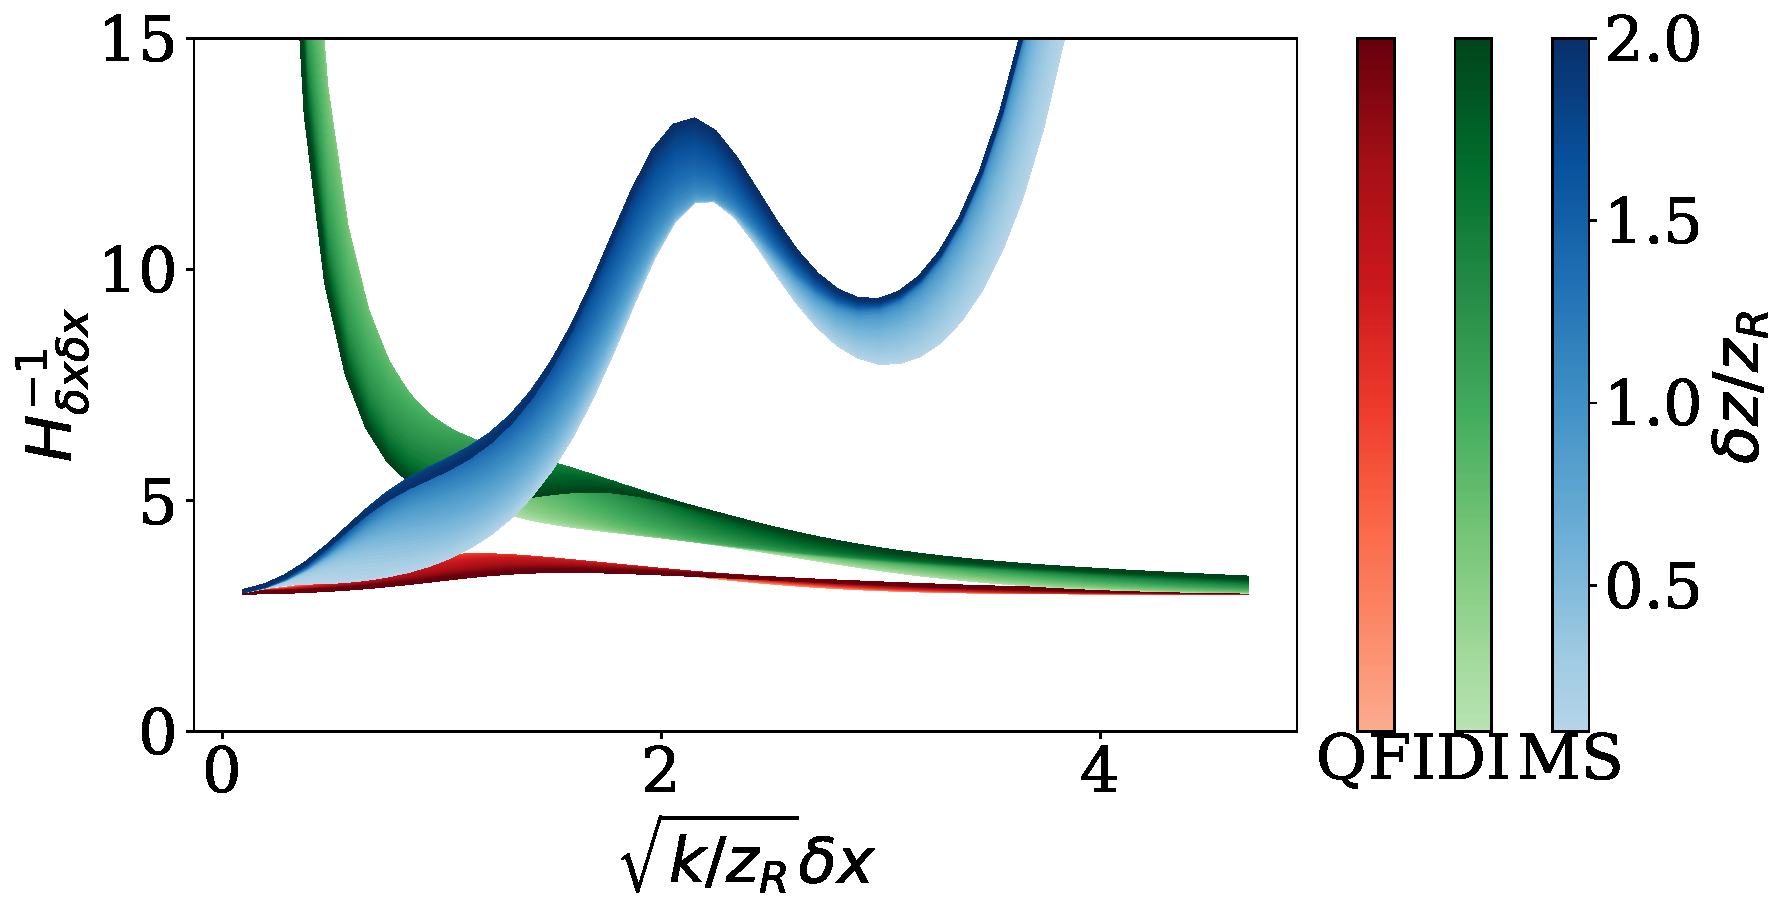
\includegraphics[height=4cm]{s_param_covariance_xy.pdf}}\\
%\subfloat[]{\label{fig:incoh_COV_p}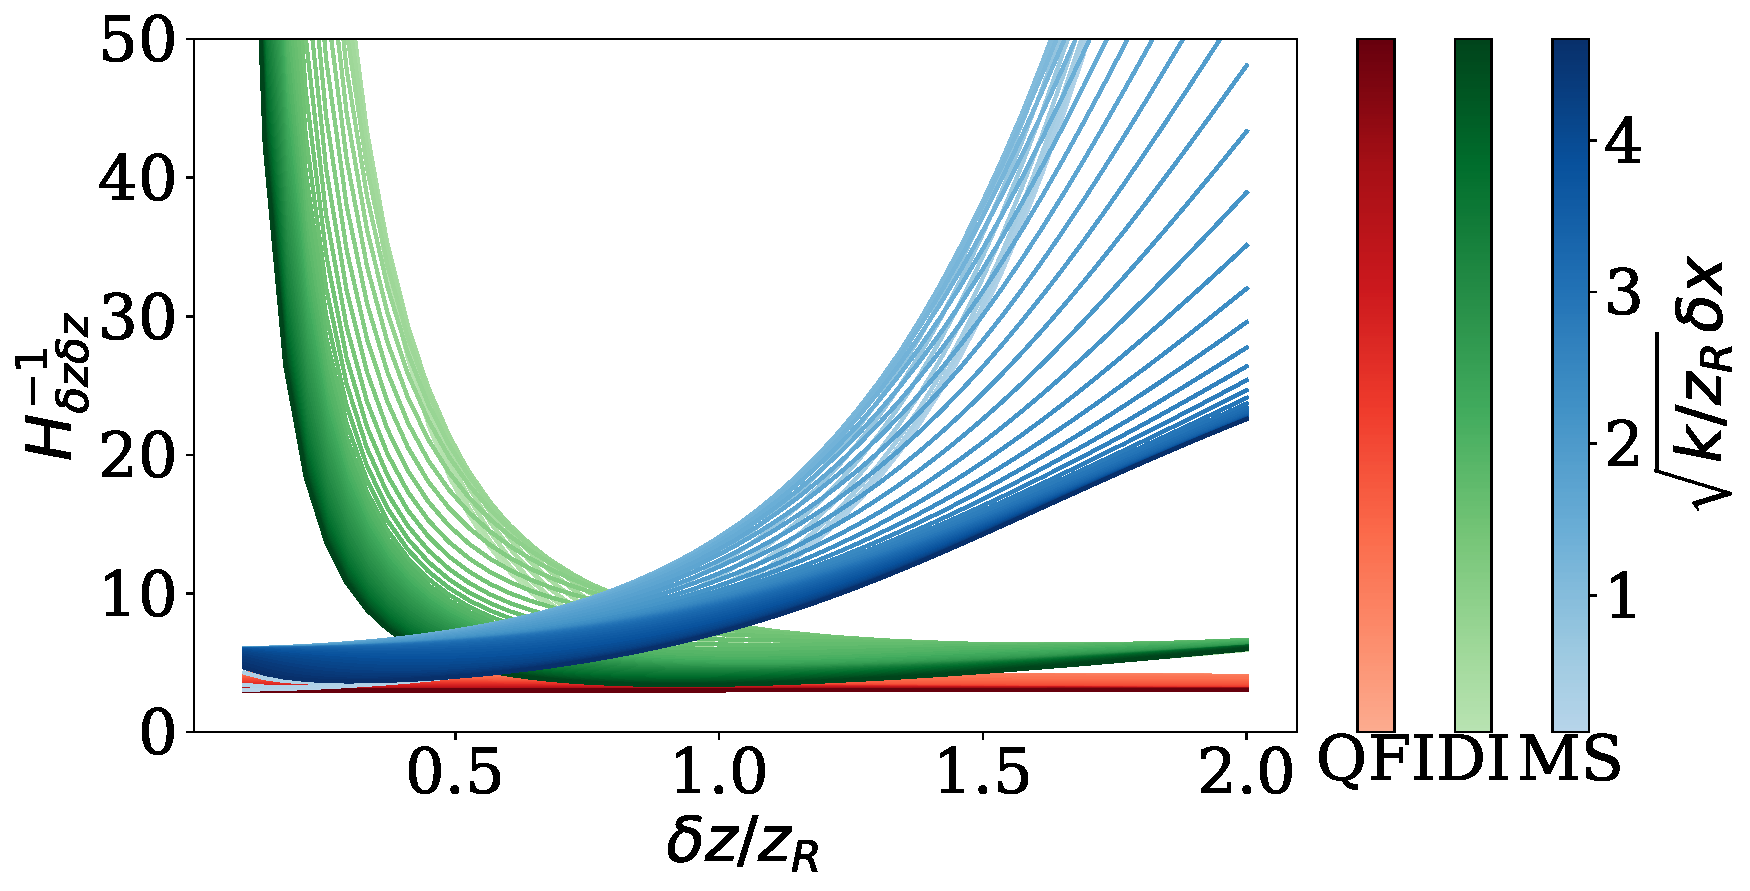
\includegraphics[height=4cm]{p_param_covariance_xy.pdf}}%
\caption{Cram\'er-Rao bounds for estimating surface crack parameters (a) $\delta x$ and (b) $\delta z$ as modelled in Fig.~\ref{fig:3source_layout}. {\color{red}MS resolves the four modes $(0,0)$, $(1,0)$, $(2,0)$, $(0,2)$ plus a remainder channel (Appendix~\ref{app:remainder}).} Red curves correspond to the ultimate quantum limit (QFI), blue curves to Hermite-Gaussian mode sorting (MS), and green curves to classical direct imaging (DI).}
\label{figshers}
\end{figure}





\paragraph{(ii) Detecting crack versus no crack.}
We now show that the techniques presented so far are also advantageous for deciding whether the object we are imaging is a crack or not. This decision problem can be characterised as a quantum hypothesis test between the images of a crack (with given width $\delta x$ and depth $\delta z$, see Fig.~\ref{fig:3source_layout}) and its absence. Let $\psi_L \equiv \psi_1$ and $\psi_R \equiv \psi_2$ be sources on the edges at $(\pm \delta x/2,0,0)$,   $\psi_C$ be on their midpoint at $(0,0,0)$ representing the centre of a flat surface, and $\psi_Z \equiv \psi_3$ be on the floor of a crack at $(0,0,-\delta z)$.
%: explicitly,
%        $\psi_L = \psi(x\!+\!\frac{\delta x}{2},y,0)$, $\psi_R = \psi(x\!-\!\frac{\delta x}{2},y,0)$, $\psi_C = \psi(x,y,0)$, $\psi_Z = \psi(x,y,-\delta z)$.
We can then define the states corresponding to each of our hypotheses.
For the null hypothesis, $\rho_0$ describes three collinear sources representing a flat surface (no crack); whereas for the alternative hypothesis, $\rho_1$ denotes a crack with depth $\delta z$,
\begin{equation}
    \begin{aligned}
        \rho_0 &= \left({\ketbra{\psi_L}{\psi_L} + \ketbra{\psi_R}{\psi_R} + \ketbra{\psi_C}{\psi_C}}\right)\!/3\,,\\
        \rho_1 &= \left({\ketbra{\psi_L}{\psi_L} + \ketbra{\psi_R}{\psi_R} + \ketbra{\psi_Z}{\psi_Z}}\right)\!/3\,.
    \end{aligned}
\end{equation}
We can now apply the definitions in Eqs.~(\ref{eq:CCB}) and (\ref{eq:QCB}) to calculate the QCB and the  Chernoff information of each measurement.


\begin{figure}
\centering
\begin{overpic}[width=7cm]{CIvsX.pdf}
    % \put(x, y) uses percentages of the image dimensions by default (0-100)
    \put(1, 3){{(a)}}
\end{overpic} \\
\vspace{0.2cm} % Optional: tweak this if you want a tiny gap between top and bottom images
\begin{overpic}[width=7cm]{CIvsZ.pdf}
    \put(1, 3){{(b)}}
\end{overpic}
\caption{Chernoff information for detecting surface cracks, plotted as a function of: (a) the width $\delta x$ for $\delta z/z_R=1$ (solid) and $0.1$ (dashed); (b) the depth $\delta z$ for $\sqrt{k/z_R}\delta_x=2$ (solid) and $0.5$ (dashed). Red curves correspond to the quantum Chernoff bound, blue curves to Hermite-Gaussian mode sorting, and green ones to direct imaging.}
\label{chernoffigo}
\end{figure}

To calculate the QCB, we take two approaches. First, a numerical approach (See Appendix~\ref{app:QCB_calculation} \cite{supposta}) with  results shown in Fig.~\ref{chernoffigo}. Second, an analytical upper bound using \cite{calsamiglia2008quantum,lupo2020quantum}
\begin{equation} \label{eq:fidelity_bound}
    \xi_Q \leq - 2 \log F(\rho_0, \rho_1),
\end{equation}
where $F(\rho_0, \rho_1) = \text{Tr}\left[ \sqrt{\sqrt{\rho_0} \rho_1 \sqrt{\rho_0}}\right]$ is the fidelity between $\rho_0$ and $\rho_1$, which we express in terms of point source overlaps in Appendix~\ref{app:QCB_calculation} \cite{supposta}. By using leading-order approximations, valid for small $\delta x$ and $\delta z$, we obtain $F(\rho_0,\rho_1) \approx 1 - \frac{\delta z^2}{24}$. We can then use Eq.~\eqref{eq:fidelity_bound} to provide a bound on the QCB,
\begin{equation}
    \xi_Q \leq \frac{\delta z^2}{12} + O(\delta z^4).
\end{equation}

We now %Having derived the quantum limit through both bounds and numerical calculations, we
turn our attention to calculating the Chernoff information Eq.~(\ref{eq:CCB}) for a classical DI intensity measurement. To do this, we first use the sum of the intensity distributions of each point source to obtain a probability distribution for each hypothesis: $P_0(x,y) = \big({|\psi_L|^2 + |\psi_R|^2 + |\psi_C|^2}\big)/{3}$ and $P_1(x,y) = \big({|\psi_L|^2 + |\psi_R|^2 + |\psi_Z|^2}\big)/{3}$. The Chernoff information for DI can then be calculated from Eq.~(\ref{eq:CCB}):
\begin{equation}\label{eq:CI_DI}
\xi_{\textrm{DI}} = - \log \min_{0 \leq s \leq 1} \mbox{$\iint P_0(x,y)^s P_1(x,y)^{1-s} dx dy$}.
\end{equation}
Like the QCB, we use numerical methods to evaluate this quantity as well as a series expansion of the integrand which is then integrated term by term to give us the leading term of the error exponent: $\xi_{\textrm{DI}} \approx - \log \min\limits_{0 \leq s \leq 1} \big( 1 - s(1-s) \frac{\delta z^4}{18}\big) = -\log \big(1 - \frac{\delta z^4}{72} \big)$.
Using the approximation $-\log(1-\epsilon) \approx \epsilon$ for $\epsilon \ll 1$, we then get the approximation $\xi_{\textrm{DI}} \approx \frac{\delta z^4}{72}$. This quartic scaling implies a severe loss of distinguishability for shallow cracks by DI compared to the quantum limit.

To benchmark MS measurements, we define $P_{j,l}(\delta x, \delta z)$ as the combined probability of detecting channel $(j,l)$ from all three point sources in a crack with given width $\delta x$ and depth $\delta z$, using Eq.~\eqref{eq:prob_ms_general}. To ensure valid probability distributions, we implicitly include a remainder channel with probability $1 - \sum_{j,l} P_{j,l}(\delta x, \delta z)$.
Noting that the null hypothesis is represented by $P_{j,l}(\delta x, 0)$,
the MS Chernoff information reads
\begin{equation} \label{eq:CI_MS}
\xi_{\textrm{MS}} = -\log \min_{0 \leq s \leq 1} \mbox{$\sum_{j,l} P_{j,l}(\delta x, 0)^s P_{j,l}(\delta x, \delta z)^{1-s}$}.
\end{equation}
As before, for MS in the Hermite-Gaussian basis we calculate this quantity numerically and give a leading-order approximation.
The approximation is obtained by noting that only four modes contain terms of second order:
		$P_{0,0}(\delta x, \delta z) \approx 1 - \frac{\delta x^2}{12} - \frac{\delta z^2}{12}$,
        $P_{1,0}(\delta x, \delta z) \approx \frac{\delta x^2}{12}$,
		$P_{2,0}(\delta x, \delta z) \approx \frac{\delta z^2}{24}$,
		$P_{0,2}(\delta x, \delta z) \approx \frac{\delta z^2}{24}$.
The channels $(2,0)$ and $(0,2)$ have particular significance as the leading-order term vanishes for a flat surface ($P_{2,0}(\delta x, 0) \approx P_{0,2}(\delta x, 0) \approx 0$) but have nonzero probability $\propto \delta z^2$ for a crack, resulting in  increased distinguishability.
By substituting our approximation into Eq.~(\ref{eq:CI_MS}), we get $\xi_{\textrm{MS}}  \approx -\log \min\limits_{0 \leq s \leq 1} \big(1  - \frac{\delta z^2}{12} + \frac{\delta z^2 s}{12} \big) \approx \frac{\delta z^2}{12}$. Since our leading order bound gives $\xi_Q \leq \frac{\delta z^2}{12}$ and $\xi_{\textrm{MS}}  \approx \frac{\delta z^2}{12}$ matches this bound, we conclude that $\xi_Q \approx \frac{\delta z^2}{12}$.

 Our hypothesis testing results, summarised in Table~\ref{tab:chernoff_comparison}, show that MS saturates the quantum limit up to second-order scaling with $\delta z$, thanks to the activation of specific channels sensitive to the crack depth. In contrast, DI produces only a small change to the intensity distribution, making shallow cracks much more difficult to distinguish from background noise.




\begin{table}[h]
\centering
\begin{tabular}{lc}
\hline \hline
\  Scheme & \qquad  Chernoff exponent \qquad  \\ \hline
\  Quantum limit (QCB) &\qquad  ${\delta z^2}/{12}$\qquad \\
\  Direct imaging (DI) &\qquad ${\delta z^4}/{72}$ \qquad\\
\  Mode sorting (MS) & \qquad ${\delta z^2}/{12}$\qquad\\ \hline \hline
\end{tabular}
\caption{Comparison of leading-order scaling of Chernoff exponents for detection of a surface crack with depth $\delta z$.}
\label{tab:chernoff_comparison}
\end{table}



\paragraph{\bfseries Conclusions.}
We have introduced a quantum statistical framework for passive optical surface metrology that unifies fundamental limits for parameter estimation and defect detection within a single description. By modelling a surface as an incoherent ensemble of point emitters imaged through a diffraction-limited system, we connected the estimability and detectability of physically meaningful surface parameters directly to Fisher information and Chernoff information bounds.
These bounds depend solely on point-spread function overlaps and their derivative structure, providing a streamlined geometric interpretation for the design of optimal measurements.

Applied to a minimal surface crack model, our analysis shows that specific spatial modes are selectively sensitive to distinct geometric features, such as crack width and depth. This enables simultaneous near-quantum-limited estimation of multiple parameters using only a small number of low-order modes, despite the absence of illumination control. Beyond estimation, the same measurement strategy markedly enhances the detection of shallow defects at the ultimate quantum limit, while classical direct imaging performs substantially worse.

Taken together, these results demonstrate that quantum-limited performance in surface metrology is, in principle, achievable with purely passive measurements in the image plane. More broadly, they show how quantum estimation and detection theory can be used not only to bound performance, but also to identify physically interpretable measurement bases tailored to specific quality control and surface analysis tasks.

% {\color{red} Because our bounds depend only on point-spread-function overlaps and their derivatives, the framework applies unchanged to non-Gaussian, aberrated, or experimentally measured PSFs, for which the overlaps are evaluated numerically rather than in closed form. On the experimental side, the cross-talk analysis in the Supplemental Material indicates that the mode-sorting advantage is robust to realistic sorter imperfections, motivating a proof-of-principle demonstration.}
{\color{red} Because our bounds depend only on point-spread-function overlaps and their derivatives, the framework applies unchanged to non-Gaussian, aberrated, or experimentally measured PSFs, for which the overlaps are evaluated numerically rather than in closed form. On the experimental side, Appendix~\ref{app:ms_errors} analyses the impact of nearest-neighbour mode cross-talk and an additive detector noise floor (from dark counts and background light) on the Fisher information. It is shown that the mode sorting remains robust to realistic imperfections, motivating a proof-of-principle demonstration.}



\begin{acknowledgments}
%We thank some people.

We are grateful to M.~Guta, H.~Hooshmand, A.~Khan, A.~Lvovsky, N.~Treps, and S.~da~Vinci for fruitful exchanges.
We acknowledge financial support from BBSRC (Grant No.~BB/X004317/1) and EPSRC (Grants No.~EP/X010929/1 and EP/Z534948/1).
\end{acknowledgments}

%\twocolumngrid
%\bibliographystyle{apsrevfixedwithtitles}
\bibliography{ref}% Produces the bibliography via BibTeX.


\clearpage
\appendix
\onecolumngrid
\setcounter{secnumdepth}{2}
\setcounter{figure}{0}
\renewcommand{\thefigure}{S\arabic{figure}}


\section*{SUPPLEMENTAL MATERIAL}

\section{Closed form Gaussian overlaps\label{app:gaussian_overlaps}}
Here we show the explicit closed form expressions of the overlaps entering the Gram matrix $G$ for a Gaussian beam,
\begin{equation}
    G_{\Delta_{v,u}} = \braket{\psi_v}{\psi_u}, \qquad    G_{\gamma^{a}_{v,u}} = \braket{\psi_v}{ \frac{\partial \psi_u}{\partial \theta_u^a}}, \qquad G_{\tau^{a,b}_{v,u}} = \braket{\frac{\partial \psi_v}{\partial \theta_v^a}}{ \frac{\partial \psi_u}{\partial \theta_u^b}}.
    \label{eq:Grammian}
\end{equation}

All overlaps share a common exponential factor
\begin{align}
    \psi_0 = \exp \left \{ (i \frac{(\delta_{x_v} - \delta_{x_u})^2 + (\delta_{y_v} - \delta_{y_u})^2)}{2(-2i + \delta_{z_v} - \delta_{z_u})} + i k z_R (\delta_{z_v} - \delta_{z_u}) \right \}.
\end{align}

We have then
\begin{align}
    \braket{\psi_v}{\psi_u} &= \frac{2 i}{2 i  - \delta_{z_v} + \delta_{z_u}} \psi_0 \\
    \braket{\partial_{\delta_{x_v}}\psi_v}{\psi_u} &=  -2 \frac{\delta_{x_v} - \delta_{x_u}}{(2i - \delta_{z_v} + \delta_{z_u})^2} \psi_0\\
    \braket{\partial_{\delta_{y_v}}\psi_v}{\psi_u} &=  -2 \frac{\delta_{y_v} - \delta_{y_u}}{(2i - \delta_{z_v} + \delta_{z_u})^2} \psi_0\\
    \braket{\partial_{\delta_{z_v}}\psi_v}{\psi_u} &= \frac{-4 + (\delta_{x_v} - \delta_{x_u})^2 + (\delta_{y_v} - \delta_{y_u})^2 - 2 k z_R (-4 + (\delta_{z_v} - \delta_{z_u})^2) +  2i (\delta_{z_v} - \delta_{z_u})  (-1 + 4 k z_R)
    }{(-2i + \delta_{z_v} - \delta_{z_u})^3} \psi_0 \\
    \braket{\partial_{\delta_{x_v}}\psi_v}{\partial_{\delta_{x_u}}\psi_u} &= \frac{2i (-2 + (\delta_{x_v} - \delta_{x_u})^2 + i (\delta_{z_u} - \delta_{z_v}))}{(2i - \delta_{z_v} + \delta_{z_u})^3} \psi_0 \\
    \braket{\partial_{\delta_{x_v}}\psi_v}{\partial_{\delta_{y_u}}\psi_u} &= \frac{2i (\delta_{x_v} - \delta_{x_u}) (\delta_{y_v} - \delta_{y_u})}{ (2i - \delta_{z_v} + \delta_{z_u})^3} \psi_0 \\
    \braket{\partial_{\delta_{x_v}}\psi_v}{\partial_{\delta_{z_u}}\psi_u} &= -\frac{(-1 + i \delta_{z_u})^3 (\delta_{x_v} - \delta_{x_u}) \psi_0}{(i + \delta_{z_u})^3 (2i - \delta_{z_v} + \delta_{z_u})^4} \\
    &(-8 + (\delta_{x_v} - \delta_{x_u})^2 + (\delta_{y_v} - \delta_{y_u})^2  - 2 k z_R (-4 + (\delta_{z_v} - \delta_{z_u})^2) + 4i (\delta_{z_v} - \delta_{z_u}) (-1 + 2 k z_R)) \nonumber \\
    \braket{\partial_{\delta_{y_v}}\psi_v}{\partial_{\delta_{y_u}}\psi_u} &= 2i \frac{-2 + (\delta_{y_v} - \delta_{y_u})^2 + i (\delta_{z_u} - \delta_{z_v})}{ (2i - \delta_{z_v} + \delta_{z_u})^3} \psi_0\\
    \braket{\partial_{\delta_{y_v}}\psi_i}{\partial_{\delta_{z_u}}\psi_u} &= - \frac{(-1 + i \delta_{z_u})^3 (\delta_{y_v} - \delta_{y_u}) \psi_0}{(i + \delta_{z_u})^3 (2i - \delta_{z_v} + \delta_{z_u})^4}  \\
    & (-8 + (\delta_{x_v} - \delta_{x_u})^2 + (\delta_{y_v} - \delta_{y_u})^2 - 2 k z_R (-4 + (\delta_{z_v} - \delta_{z_u})^2) + 4i (\delta_{z_v} - \delta_{z_u}) (-1 + 2 k z_R)) \nonumber \\
    \braket{\partial_{\delta_{z_v}}\psi_v}{\partial_{\delta_{z_u}}\psi_u} &= \frac{i \psi_0}{2 (-2i + \delta_{z_v} - \delta_{z_u})^5} \bigg(  \\
    & -32 + 8 (\delta_{z_v} - \delta_{z_u})^2 - (\delta_{x_v} - \delta_{x_u})^2 ((\delta_{x_v} - \delta_{x_u})^2 + 2 (-8 + (\delta_{y_v} - \delta_{y_u})^2)) -(\delta_{y_v} - \delta_{y_u})^2 (-16 + (\delta_{y_v} - \delta_{y_u})^2) \nonumber \\
    &  + 64 k z_R + 4 k z_R
        (
            (\delta_{z_v} - \delta_{z_u})^2 (-12 + (\delta_{x_v} - \delta_{x_u})^2 + (\delta_{y_v} - \delta_{y_u})^2)
            - 4 ((\delta_{x_v} - \delta_{x_u})^2 + (\delta_{y_v} - \delta_{y_u})^2)
        ) \nonumber \\
    &- (2 k z_R)^2
        (
            (-4 + 4 \delta_{z_v} + \delta_{z_v}^2 - 2 (2 + \delta_{z_v}) \delta_{z_u} + \delta_{z_u}^2)
            (-4 + \delta_{z_v}^2 - 2 \delta_{z_v} (2 + \delta_{z_u}) + \delta_{z_u} (4 + \delta_{z_u}))
        ) \nonumber \\
    &+ i
        (8 (\delta_{z_v} - \delta_{z_u}) ( -4 + (\delta_{x_v} - \delta_{x_u})^2 + (\delta_{y_v} - \delta_{y_u})^2 - k z_R (-12 + (\delta_{z_v} - \delta_{z_u})^2) \nonumber \\
        &- 2 k z_R ((\delta_{x_v} - \delta_{x_u})^2 + (\delta_{y_v} - \delta_{y_u})^2) + (2 k z_R)^2 (-4 + (\delta_{z_v} - \delta_{z_u})^2)))\bigg)\nonumber
\end{align}

\section{Derivation of the Quantum Fisher Information Matrix\label{app:qfi_derivation}}
We will derive the final QFIM expression Eq.~\eqref{eq:qfim_final} in two steps. Firstly, let us show that the elements are fully determined by the Gram matrix Eq.~(\ref{eq:Grammian})
and first-quadrant SLDs Eq.~\eqref{eq:L_delta_sylvester}. Writing the SLD in the same matrix block form as Eq.~(\ref{eatlean}), we can compute the Lyapunov equation Eq.~\eqref{eq:sld_nonorthogonal}
\begin{align}
    2 \begin{pmatrix}
        0 & \Tilde{D}_\gamma \\
        \Tilde{D}_{\gamma^\dagger} & 0
    \end{pmatrix} = \begin{pmatrix}
        \openone_V & 0 \\
        0 & 0
    \end{pmatrix} \begin{pmatrix}
        G_\Delta & G_\gamma \\
        G_{\gamma^\dagger} & G_{\tau}
    \end{pmatrix} \begin{pmatrix}
        L_\Delta & L_\gamma \\
        L_{\gamma^\dagger} & L_{\tau}
    \end{pmatrix} + \begin{pmatrix}
        L_\Delta & L_\gamma \\
        L_{\gamma^\dagger} & L_{\tau}
    \end{pmatrix} \begin{pmatrix}
        G_\Delta & G_\gamma \\
        G_{\gamma^\dagger} & G_{\tau}
    \end{pmatrix} \begin{pmatrix}
        \openone_V & 0 \\
        0 & 0
    \end{pmatrix},
\end{align}
where for brevity we omit the parameter index $a$, and we can cancel the $1/V$ factor of the density matrix $V R$ on the right hand side and the derivative matrix $\Tilde{D} = V D$ on the left hand side. Performing the multiplication leads to
\begin{align}
    2 \begin{pmatrix}
        0 & \Tilde{D}_\gamma \\
        \Tilde{D}_{\gamma^\dagger} & 0
    \end{pmatrix} = \begin{pmatrix}
        G_\Delta L_\Delta + L_\Delta G_\Delta + G_\gamma L_{\gamma^\dagger} + L_\gamma G_{\gamma^\dagger} & G_\Delta L_\gamma + G_\gamma L_\tau \\
        L_{\gamma^\dagger} G_\Delta + L_\tau G_{\gamma^\dagger} & 0
    \end{pmatrix}.
\end{align}
Since $R$ only spans support on the first quadrant $\Delta$ subspace, we can without loss of generality set $L_{\tau} = 0$ because the SLD is only defined on the support of $R$, and any component acting outside the support does not affect the QFIM \cite{liu2020quantum}. By element-wise comparison we obtain three matrix equations
\begin{align}
    2 \Tilde{D}_\gamma &= G_\Delta L_\gamma \\
    2 \Tilde{D}_{\gamma^\dagger} &= L_{\gamma^\dagger} G_\Delta \\
    0 & = G_\Delta L_\Delta + L_\Delta G_\Delta + G_\gamma L_{\gamma^\dagger} + L_\gamma G_{\gamma^\dagger}.\label{eq:reduced_sylvester}
\end{align}
Due to our basis construction, the Gram sub-matrix is invertible. Let us write the inverse of $G_\Delta$ as $G^{-1}_\Delta$, then we can formally solve for $L_\gamma$ and $L_{\gamma^\dagger}$ and insert them into Eq.~\eqref{eq:reduced_sylvester} to obtain Eq.~\eqref{eq:L_delta_sylvester}.

Secondly, to derive the QFIM expression we will begin with the definition Eq.~\eqref{eq:qfi_nonorthogonal} and note that due to the properties of computing the trace of a matrix we only need to compute the first quadrant $\Delta$ and fourth quadrant $\tau$, which results in
\begin{align}
    H_{a,b} = \Re \Tr (L_a G D_b G) &= \Re \bigg[\Tr (L^a_\Delta G_\Delta D^b_\gamma G_{\gamma^\dagger}) + \Tr (L^a_\gamma G_{\gamma^\dagger} D^b_\gamma G_{\gamma^\dagger}) + \Tr (L^a_{\Delta} G_{\gamma} D^b_{\gamma^\dagger} G_\Delta) \nonumber \\ &\quad\quad\ +
    \Tr (L^a_{\gamma} G_\tau D^b_{\gamma^\dagger} G_\Delta)
    + \Tr (L^a_{\gamma^\dagger} G_\Delta D^b_{\gamma} G_\tau)
    + \Tr (L^a_{\gamma^\dagger} G_{\gamma} D^b_{\gamma^\dagger} G_{\gamma}) \bigg].
\end{align}
We can permute the arguments of a trace, substitute again for $L_\gamma, L_{\gamma^\dagger}$ and write out explicitly the derivative matrices
\begin{align}
    H_{a,b} &= \Re \bigg[
     \Tr (L^a_\Delta G_\Delta \ket{\gamma^b}\bra{\gamma^b} G_{\gamma^\dagger})
    +  \Tr (2 G^{-1}_\Delta\ket{\gamma^{a}}\bra{\gamma^{a}} G_{\gamma^\dagger} \ket{\gamma^b}\bra{\gamma^b} G_{\gamma^\dagger})
    +  \Tr (L^a_{\Delta} G_{\gamma} \ket{\gamma^{b\dagger}}\bra{\gamma^{b\dagger}} G_\Delta) \nonumber  \\
    &\quad\qquad + \Tr (2 \ket{\gamma^a}\bra{\gamma^a} G_\tau \ket{\gamma^{b\dagger}}\bra{\gamma^{b\dagger}})
    +  \Tr (2\ket{\gamma^{a\dagger}}\bra{\gamma^{a\dagger}} G_\Delta \ket{\gamma^b}\bra{\gamma^b})
    +  \Tr (2\ket{\gamma^{a\dagger}}\bra{\gamma^{a\dagger}}G^{-1}_\Delta G_{\gamma} \ket{\gamma^{b\dagger}}\bra{\gamma^{b\dagger}} G_{\gamma})
 \bigg] \nonumber \\
    &= \Re \bigg[
    \bra{\gamma^b} G_{\gamma^\dagger} L^a_\Delta G_\Delta\ket{\gamma^b}
    +  2 \bra{\gamma^{a}}G_{\gamma^\dagger}\ket{\gamma^b} \bra{\gamma^b} G_{\gamma^\dagger} G^{-1}_\Delta  \ket{\gamma^{a}}
\nonumber    \\ & \quad\qquad+  \bra{\gamma^{b\dagger}} G_\Delta L^a_{\Delta} G_{\gamma} \ket{\gamma^{b\dagger}}  + 2\bra{\gamma^{b\dagger}} G_{\gamma} \ket{\gamma^{a\dagger}}\bra{\gamma^{a\dagger}}G^{-1}_\Delta G_{\gamma}\ket{\gamma^{b\dagger}} \bigg]\nonumber \\
    &= 2\Re \bra{\gamma^b} G_{\gamma^\dagger} L^a_\Delta G_\Delta \ket{\gamma^b}
    + 4 \Re \bra{\gamma^a}G_{\gamma^\dagger}\ket{\gamma^b}\bra{\gamma^b}G_{\gamma^\dagger} G^{-1}_\Delta\ket{\gamma^a},
\end{align}
where in the first step we use the sparsity to reduce the trace to an inner product and in the second step the Hermitian property of all the operators to combine terms.

\section{Classical Fisher Information for an arbitrary polynomial measurement basis\label{app:ms_incoherent}}
To calculate the FIM for a mode measurement Eq.~\eqref{eq:FI_MS}, we first represent the object as an arbitrary discrete distribution of $V$ point sources
\begin{align}
    F(r|\theta) = \frac{1}{V} \sum_v^V \delta \left [ x + \delta x_v, y + \delta y_v, \delta z_v \right ],
\end{align}
with $\delta[x]$ the Dirac delta. Defining the object distribution via a sum of Dirac delta functions simplifies calculating the measurement channel probabilities to Eq.~\eqref{eq:prob_ms_general}.

For each measurement channel contribution $\frac{1}{P_j(\theta)} \pdv{P_j(\theta)}{\theta_a}  \pdv{P_j(\theta)}$ to the FIM Eq.~\eqref{eq:FI_MS} we need to compute and sum the individual measurement mode probabilities for a single source $\abs{ \braket{\phi_{j,l}}{\psi_v(x + \delta x_v, y + \delta y_v, \delta z_v)} }^2$. However, due to construction, calculating the measurement mode sensitivity for a specific point source displacement only involves computing the single source measurement probability derivative
\begin{align}
 \!\!   \pdv{P_{j,l}(\theta)}{\theta_v^a} &= \frac{1}{V} \pdv{}{\theta_v^a} \abs{\braket{\phi_{j,l}}{\psi(x + \delta x_v, y + \delta y_v, \delta z_v)}}^2.
 \label{eq:pdv_mode_dot_product}
\end{align}
We assume the modes to be a point-spread function adapted basis \cite{rehacek2017optimal} expressed as \begin{align}
    \phi_{j,l}(x,y) = g_j(x)f_l(y)\psi(x,y,0) = \sum_\zeta^j \sum_\xi^l c^*_\zeta d^*_\xi x^\zeta y^\xi \sqrt{\frac{1}{\pi}} \exp{-\frac{(x^2 + y^2)}{2}},
\end{align}
where $g_j(x)$ (resp.~$f_l(y)$) are polynomials of order $j$ (resp.~$l$) separable in $xy$-dimensions. The measurement overlap between the point source distribution and our measuring mode becomes

\begin{align}
    &\braket{\phi_{j,l}}{\psi(x+\delta_x,y+\delta_y,\delta_z)} = \iint dxdy \  g^*_j(x) \ f^*_l(y) \ \psi(x,y,0) \ \psi(x+\delta_x,y+\delta_y,\delta_z) \nonumber \\
     &= \iint dxdy \ \left [  \sum_\zeta^j \sum_\xi^l c^*_\zeta d^*_\xi x^\zeta y^\xi \sqrt{\frac{1}{\pi}} \exp{-\frac{(x^2 + y^2)}{2}} \right ]^* \sqrt{\frac{1}{\pi}} \frac{i}{i + \delta_z}\exp{-i\frac{((x+\delta_x)^2 + (y+\delta_y)^2)}{2(i+\delta_z)} - i k z_R \delta_z} \nonumber \\
     &= \sum_\zeta^j  \sum_\xi^l c_\zeta^*  d_\xi^* \frac{1}{\pi} \frac{i \exp{-ikz_R \delta_z} \exp{\frac{-i( \delta_x^2 + \delta_y^2)}{2(2i+\delta_z)}}}{i+\delta_z} \int dx \ x^\zeta \exp{-\frac{(x - \mu_x)^2}{2\sigma_z^2}} \int dy \ y^\xi \exp{-\frac{(y - \mu_y)^2}{2\sigma_z^2}},
\end{align}
with $\mu_x = -i\delta_x / (2i + \delta_z), \mu_y = -i\delta_y / (2i + \delta_z)$, and $\frac{1}{2\sigma_z^2} = \frac{1}{2} [ 1 + \frac{i}{i + \delta_z}]$. We can use the formula for complex-valued Gaussian integrals,
\begin{align}
    \int dx \ \exp{-ax^2} = \sqrt{\frac{\pi}{a}}
\end{align}
since $\Re{a} \geq 0$ will always hold. We can now express each integral as the generating functions of the moments for a normal distribution and obtain the result
\begin{align}
   \braket{\phi_{j,l}}{\psi(x+\delta_x,y+\delta_y,\delta_z)} &= \frac{2i}{2i + \delta_z}  \exp{-ikz_R\delta_z} \exp{-\frac{i}{2(2i +\delta_z)}(\delta_x^2 + \delta_y^2)} \sum_\zeta^j c^*_\zeta \mathbb{E}[x^\zeta]\sum_\xi^l d^*_\xi \mathbb{E}[y^\xi],
\end{align}
with $\mathbb{E}[x_v^\zeta]$ (resp. $\mathbb{E}[y_v^\xi]$) the moments of the Gaussian distribution that can be computed recursively via
\begin{align}
    \label{def:recursive_moments}
    &\mathbb{E}[x_v^{\zeta+1}] = \mu_{x_v} \mathbb{E}[x_v^\zeta] + \zeta \sigma_{z_v}^2 \mathbb{E}[x_v^{\zeta-1}], \\
    &\mathbb{E}[x_v^0] = 1,  \quad \mathbb{E}[x_v^1] = \mu_{x_v} \nonumber.
\end{align}
Taking the absolute square of the inner product leads to the single source measurement probability
\begin{align}
\label{eq:three_sources_incoherent_ms_prob}
    \abs{\braket{\phi_{j,l}}{\psi(x + \delta x_v, y + \delta y_v, \delta z_v)}}^2 = \frac{4}{4 + \delta z_v^2} \exp{-2 \frac{\delta x_v^2 + \delta y_v^2}{4+\delta z_v^2}} \mbox{$\abs{\sum_\zeta^j c^*_\zeta \mathbb{E}[x_v^\zeta]}^2$} \mbox{$\abs{\sum_\xi^l d^*_\xi \mathbb{E}[y_v^\xi]}^2$}.
\end{align}
We can further reduce deriving the derivatives w.r.t. the point source displacements $(\delta_x,\delta_y,\delta_z)$ Eq.~\eqref{eq:pdv_mode_dot_product}
\begin{align}
    \frac{\partial}{\partial_\theta} \abs{\braket{\phi_{j,l}}{\psi(x+\delta_x,y+\delta_y,\delta_z)}}^2 &= \left ( \frac{\partial}{\partial_\theta} \braket{\phi_{j,l}}{\psi(x+\delta_x,y+\delta_y,\delta_z)}^*\right ) \braket{\phi_{j,l}}{\psi(x+\delta_x,y+\delta_y,\delta_z)} \nonumber \\
    &+ \braket{\phi_{j,l}}{\psi(x+\delta_x,y+\delta_y,\delta_z)}^* \frac{\partial}{\partial_\theta} \braket{\phi_{j,l}}{\psi(x+\delta_x,y+\delta_y,\delta_z)}
\end{align}
to computing the derivative of the inner product. We first centralise the random variable $x \sim \cal{N} (\mu,\sigma^2)$ by $x=\mu + \sigma Z$, where $Z \sim \cal{N}$$(0,1)$ and re-express the recurrence relation Eq.~\eqref{def:recursive_moments} as a sum
\begin{align}
    \mathbb{E}[x^\zeta] = \mathbb{E}[(\mu + \sigma Z)^\zeta] = \sum_\alpha^\zeta \binom{\zeta}{\alpha} \mu^\alpha \sigma^{\zeta-\alpha} \mathbb{E}[Z^{\zeta-\alpha}],
\end{align}
where
\begin{align}
    \mathbb{E}[Z^{\zeta-\alpha}] = \begin{cases}
        \frac{(\zeta-\alpha)!}{2^{\frac{\zeta-\alpha}{2}} (\frac{\zeta-\alpha}{2})!} & \zeta-\alpha \text{ is even} \\
        0 & \text{else}
    \end{cases}.
\end{align}
The individual derivatives of the measurement mode overlap have the closed form expressions
\begin{align}
    \frac{\partial}{\partial \delta_x} \braket{\phi_{j,l}}{\psi(x+\delta_x,y+\delta_y,\delta_z)} &= \frac{2i}{2i + \delta_z}  \exp{-ikz_R\delta_z} \exp{-\frac{i \delta_y^2}{2(2i +\delta_z)}} \sum_\xi^l d^*_\xi \mathbb{E}[y^\xi]\sum_\zeta c^*_\zeta  \frac{\partial}{\partial \delta_x} \left [ \exp{-\frac{i\delta_x^2}{2(2i +\delta_z)}}\mathbb{E}[x^\zeta] \right ] \nonumber \\
    &=  \frac{2}{(2i + \delta_z)^2}  \exp{-ikz_R\delta_z} \exp{-\frac{i (\delta_x^2 + \delta_y^2)}{2(2i +\delta_z)}} \left ( \sum_\xi^l d^*_\xi \mathbb{E}[y^\xi] \right ) \left [ \delta_x \sum_\zeta c^*_\zeta \mathbb{E}[x^\zeta] \right. \nonumber \\
    & \left. + \sum_\zeta c^*_\zeta \sum^\zeta_\alpha \binom{\zeta}{\alpha} \alpha \mu_x^{\alpha-1} \sigma^{\frac{\zeta-\alpha}{2}}  \mathbb{E}[Z^{\zeta-\alpha}] \right ].
\end{align}
Similarly, by symmetry, we get the expression for the derivative in the $y$-dimension
\begin{align}
    \frac{\partial}{\partial \delta_y} \braket{\phi_{j,l}}{\psi(x+\delta_x,y+\delta_y,\delta_z)} &=  \frac{2}{(2i + \delta_z)^2}  \exp{-ikz_R\delta_z} \exp{-\frac{i (\delta_x^2 + \delta_y^2)}{2(2i +\delta_z)}} \left ( \sum_\zeta^j c^*_\zeta \mathbb{E}[x^\zeta] \right ) \left [ \delta_y \sum_\xi d^*_\xi \mathbb{E}[y^\xi] \right. \nonumber \\
    & \left. + \sum_\xi d^*_\xi \sum^\xi_\beta \binom{\xi}{\beta} \beta \mu_y^{\beta-1} \sigma^{\frac{\xi-\beta}{2}}  \mathbb{E}[Z^{\xi-\beta}] \right ].
\end{align}
Lastly, we have
\begin{align}
    \frac{\partial}{\partial \delta_z} &\braket{\phi_{j,l}}{\psi(x+\delta_x,y+\delta_y,\delta_z)} = \nonumber \\
    &\sum_\zeta^j c^*_\zeta \mathbb{E}[x^\zeta]\sum_\xi^l d^*_\xi \mathbb{E}[y^\xi] \frac{\partial}{\partial \delta_z} \left [ \frac{2i}{2i + \delta_z}  \exp{-ikz_R\delta_z} \exp{-\frac{i (\delta_x^2 + \delta_y^2)}{2(2i +\delta_z)}}  \right] \nonumber \\
    &+ \frac{2i}{2i + \delta_z}  \exp{-ikz_R\delta_z} \exp{-\frac{i (\delta_x^2 + \delta_y^2)}{2(2i +\delta_z)}} \frac{\partial}{\partial \delta_z} \left[ \sum_\zeta^j c^*_\zeta \mathbb{E}[x^\zeta]\sum_\xi^l d^*_\xi \mathbb{E}[y^\xi] \right] \nonumber \\
    &= \frac{4 - \delta_x^2 - \delta_y^2 -2i\delta_z + 2k z_R(2i+\delta_z)^2}{(2i + \delta_z)^3}\exp{-i k z_R \delta_z} \exp{-\frac{\delta_x^2 + \delta_y^2}{2(2i + \delta_z)}} \sum_\zeta^j c^*_\zeta \mathbb{E}[x^\zeta]\sum_\xi^l d^*_\xi \mathbb{E}[y^\xi] \nonumber \\
    &+ \frac{2i}{2i + \delta_z} \exp{-i k z_R \delta_z} \exp{-\frac{\delta_x^2 + \delta_y^2}{2(2i + \delta_z)}} \nonumber \\
    &\left [ \left ( \sum_\xi^l d_\xi^* \mathbb{E}[y^\xi] \right ) \sum_\zeta^j c^*_\zeta \sum_\alpha^\zeta \binom{\zeta}{\alpha} \frac{(\zeta - \alpha)!}{2^{\frac{\zeta-\alpha}{2}}(\frac{\zeta-\alpha}{2})!} \frac{i}{(2i+\delta_z)^2} \left ( \frac{\zeta - \alpha}{2} \mu_x^\alpha \sigma^{\frac{\zeta - \alpha}{2}-1} + \delta_x \alpha \mu_x^{\alpha-1}  \sigma^{\frac{\zeta - \alpha}{2}} \right ) \right ] \nonumber \\
    &+ \left [ \left ( \sum_\zeta^j c_\zeta^* \mathbb{E}[x^\zeta] \right ) \sum_\xi^l d^*_\xi \sum_\beta^\xi \binom{\xi}{\beta} \frac{(\xi - \beta)!}{2^{\frac{\xi-\beta}{2}}(\frac{\xi-\beta}{2})!} \frac{i}{(2i+\delta_z)^2} \left ( \frac{\xi - \beta}{2} \mu_y^\beta \sigma^{\frac{\xi - \beta}{2}-1} + \delta_y \beta \mu_y^{\beta-1}  \sigma^{\frac{\xi - \beta}{2}} \right ) \right ].
\end{align}

As an example, the Fisher information matrix elements for the estimation of the depth and width parameters of a surface crack modelled as in Fig.~1 of the main text are plotted in Fig.~\ref{fig:supp4figs}


\begin{figure*}[h]
\centering
\subfloat[Fisher information for the estimation of the width parameter $\delta x$.]{\label{fig:incoh_FI_s}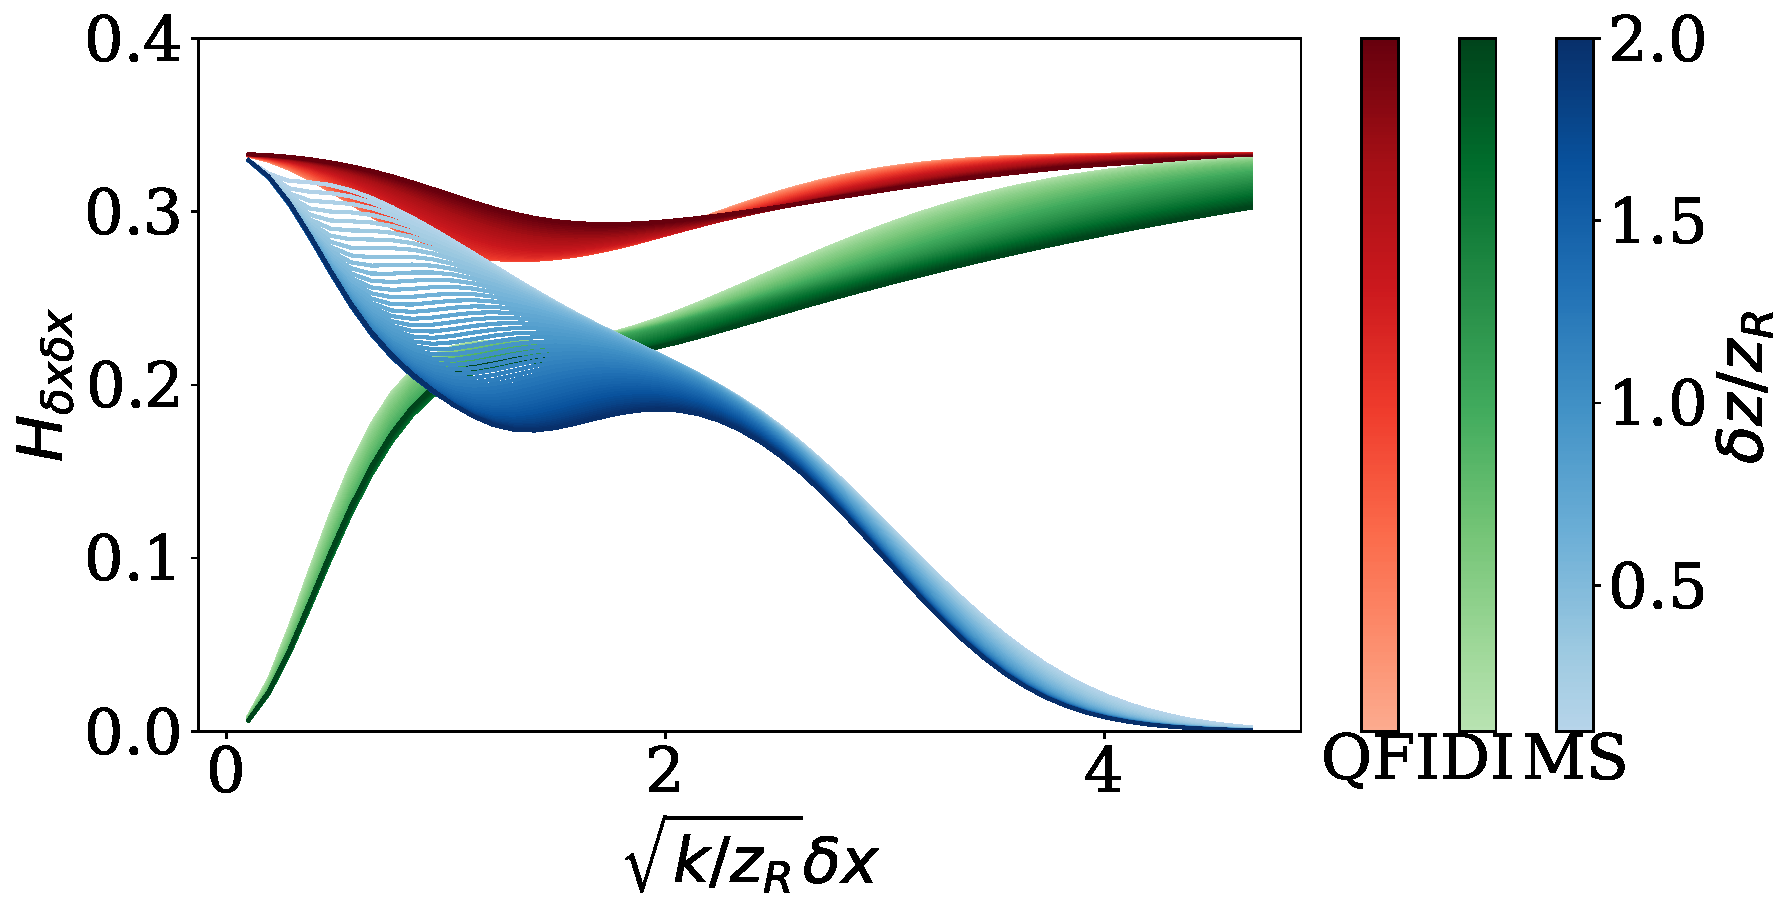
\includegraphics[width=0.45\columnwidth]{s_param_fi_comparison_optimal_remainder.pdf}}\qquad
\subfloat[Individual mode contributions to the Fisher information for the estimation of the width parameter $\delta x$.]{\label{fig:incoh_MS_s}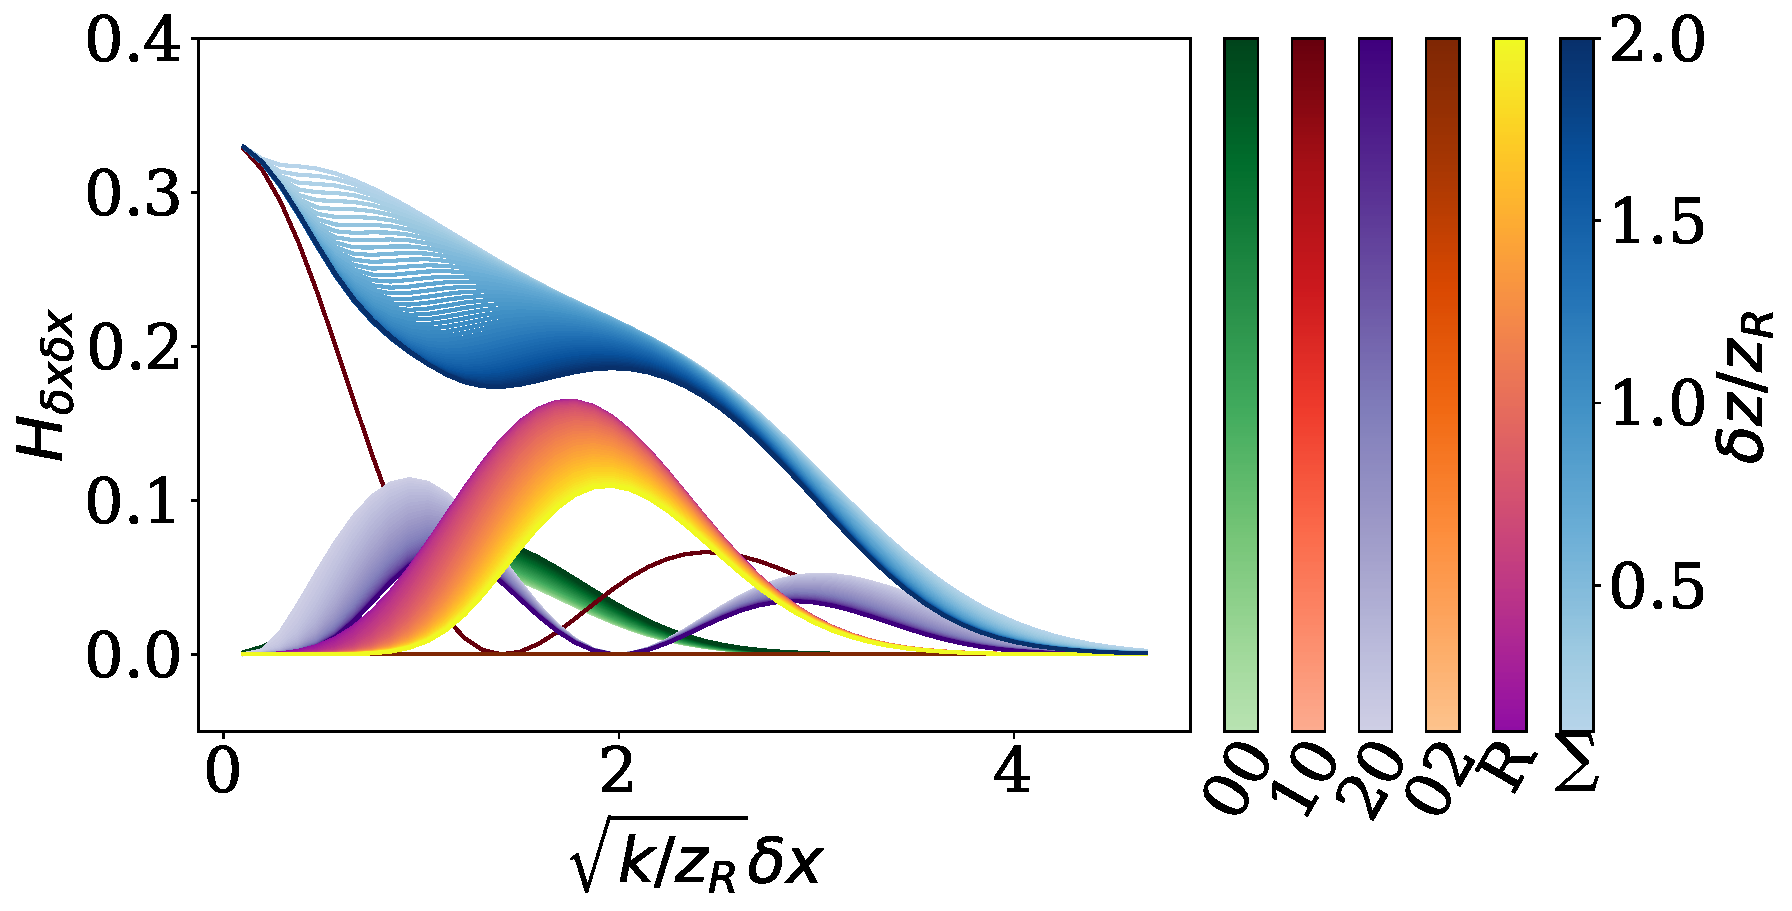
\includegraphics[width=0.45\columnwidth]{s_param_individual_mode_contributions_optimal_remainder.pdf}}\\
\subfloat[Fisher information for the estimation of the depth parameter $\delta z$.]{\label{fig:incoh_FI_p}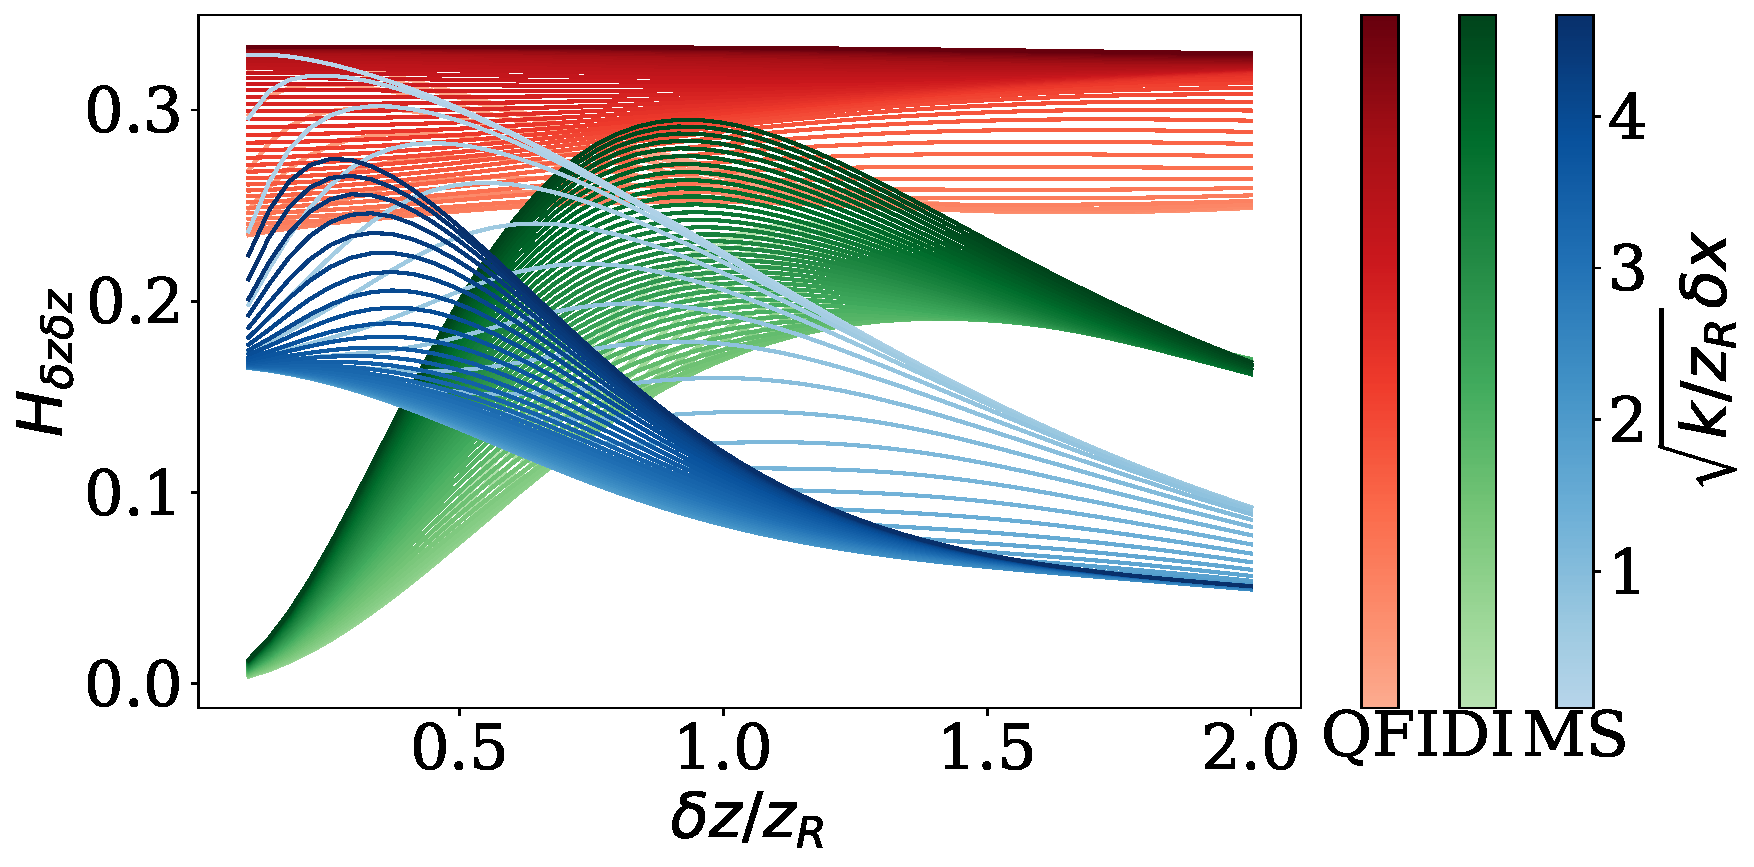
\includegraphics[width=0.45\columnwidth]{p_param_fi_comparison_optimal_remainder.pdf}}\qquad
\subfloat[Individual mode contributions to the Fisher information for the estimation of the depth parameter $\delta z$.]{\label{fig:incoh_MS_p}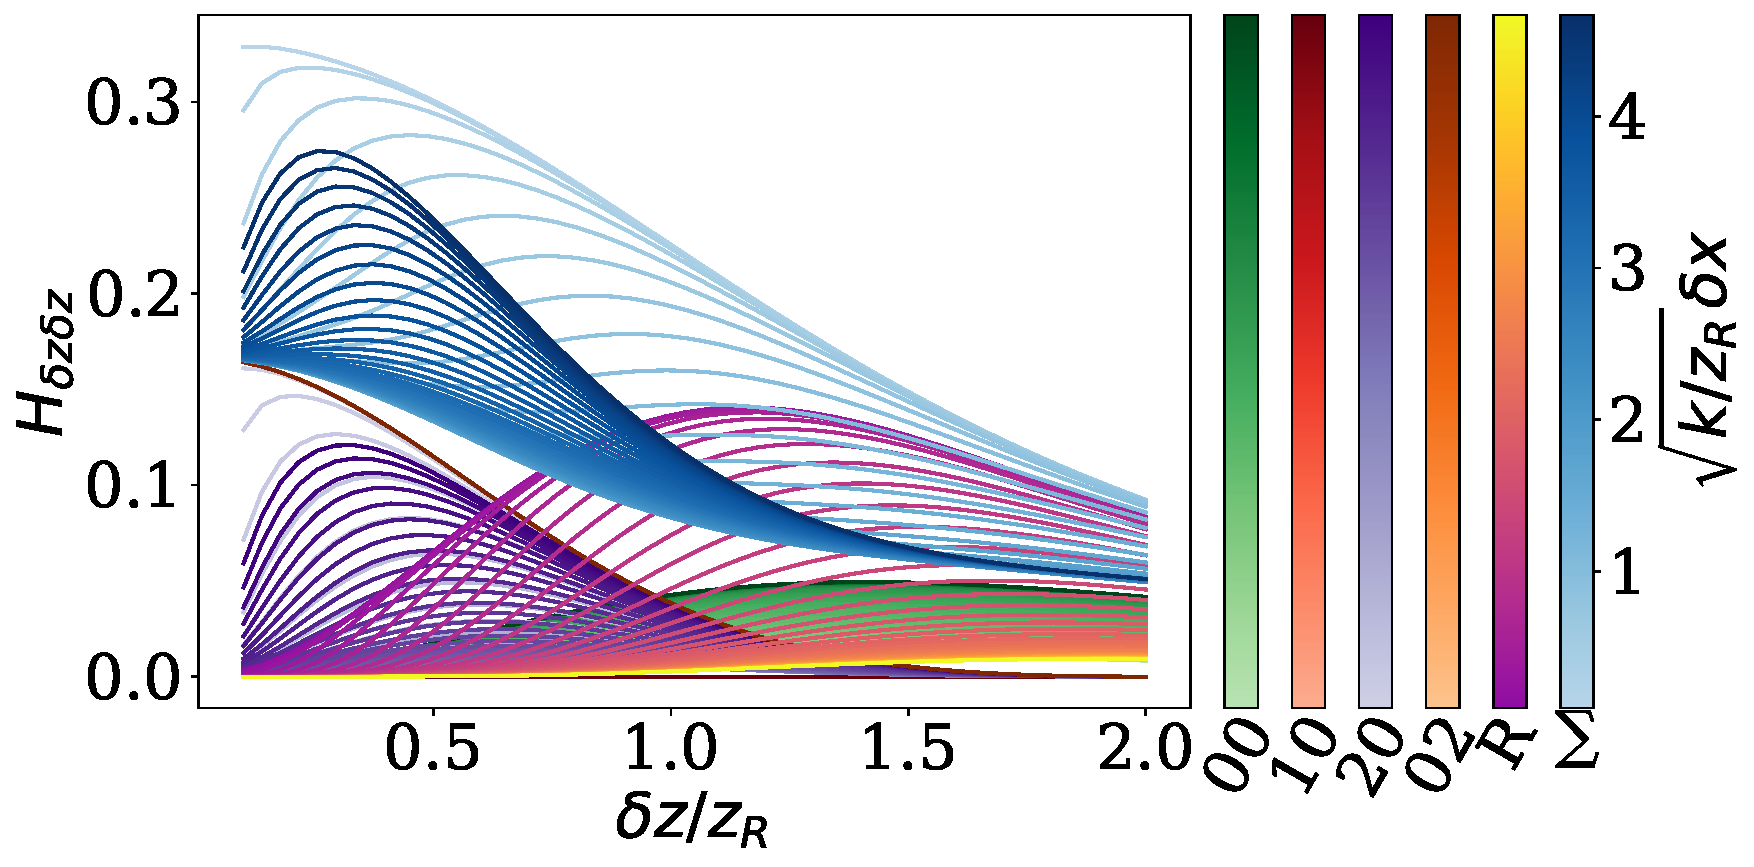
\includegraphics[width=0.45\columnwidth]{p_param_individual_mode_contributions_optimal_remainder.pdf}}%
\caption{Estimation of the parameters $\delta x$ [(a),(b)] and $\delta z$ [(c),(d)], for the incoherent three-source crack model depicted in Fig.~1 of the main text. Contributions of Hermite-Gaussian modes to the Fisher Information (Blue - MS), compared to the Quantum Fisher Information (Red - QFI) and the classical intensity measurement (Green - DI) [(a),(c)]. Individual Hermite-Gaussian modes with $(i,j)$ the 2D Hermite polynomial order,
% where for brevity we combine all the modes where the FIM matrix element is 0 (Brown - ij) and the last column is the sum of all the modes (Blue - $\sum$) [(b),(d)].
{\color{red}where the remainder channel (Pink-Yellow - $R$), collecting all unresolved light, is shown explicitly (Appendix~\ref{app:remainder}) and the last column is the sum of all channels (Blue - $\sum$) [(b),(d)].}
}
\label{fig:supp4figs}
\end{figure*}


\section{{\color{red}The remainder channel}\label{app:remainder}}
{\color{red}
A mode sorter resolves only a set $\mathcal{M}$ of Hermite-Gaussian modes. As these modes are complete, the unresolved light forms a single positive outcome $\Pi_{\rm rem}=\openone-\sum_{(j,l)\in\mathcal{M}}\Pi_{j,l}$, so $\{\Pi_{j,l}\}_{\mathcal{M}}\cup\{\Pi_{\rm rem}\}$ is a complete POVM with remainder probability
\begin{equation}
P_{\rm rem}(\theta)=1-\sum_{(j,l)\in\mathcal{M}}P_{j,l}(\theta).
\label{eq:rem_prob}
\end{equation}
Physically $\Pi_{\rm rem}$ is the dump port of a realistic mode sorter, so the measurement accounts for every photon in the image plane. This is the same remainder channel used for detection [cf.\ Eq.~\eqref{eq:CI_MS}].

As the classical Fisher information is additive over outcomes, the remainder adds a single term to Eq.~\eqref{eq:FI_MS},
\begin{equation}
J_{ab}=\tau\left[\sum_{(j,l)\in\mathcal{M}}\frac{\partial_a P_{j,l}\,\partial_b P_{j,l}}{P_{j,l}}+\frac{\partial_a P_{\rm rem}\,\partial_b P_{\rm rem}}{P_{\rm rem}}\right],\qquad \partial_a P_{\rm rem}=-\sum_{(j,l)\in\mathcal{M}}\partial_a P_{j,l}.
\label{eq:rem_fi}
\end{equation}

The leaked fraction $P_{\rm rem}$ measures the collected light that is not resolved; this is measurement-design completeness and should not be conflated with optical loss. In the sub-Rayleigh regime, essentially all photons and information are captured in the dominant four modes [Fig.~\ref{fig:crb_convergence}] --- sorting leads to probabilities summing to unity up to second order ($P_{0,0}\approx1-\tfrac{\delta x^2}{12}-\tfrac{\delta z^2}{12}$, $P_{1,0}\approx\tfrac{\delta x^2}{12}$, $P_{2,0}\approx P_{0,2}\approx\tfrac{\delta z^2}{24}$) [Fig.~\ref{fig:leaked_fraction}]. Hence, the remainder channel $P_{\rm rem}=O(\delta^4)$ is negligible and improves the bound only beyond the Rayleigh length, where direct imaging already attains the quantum limit.

\begin{figure*}[h]
\centering
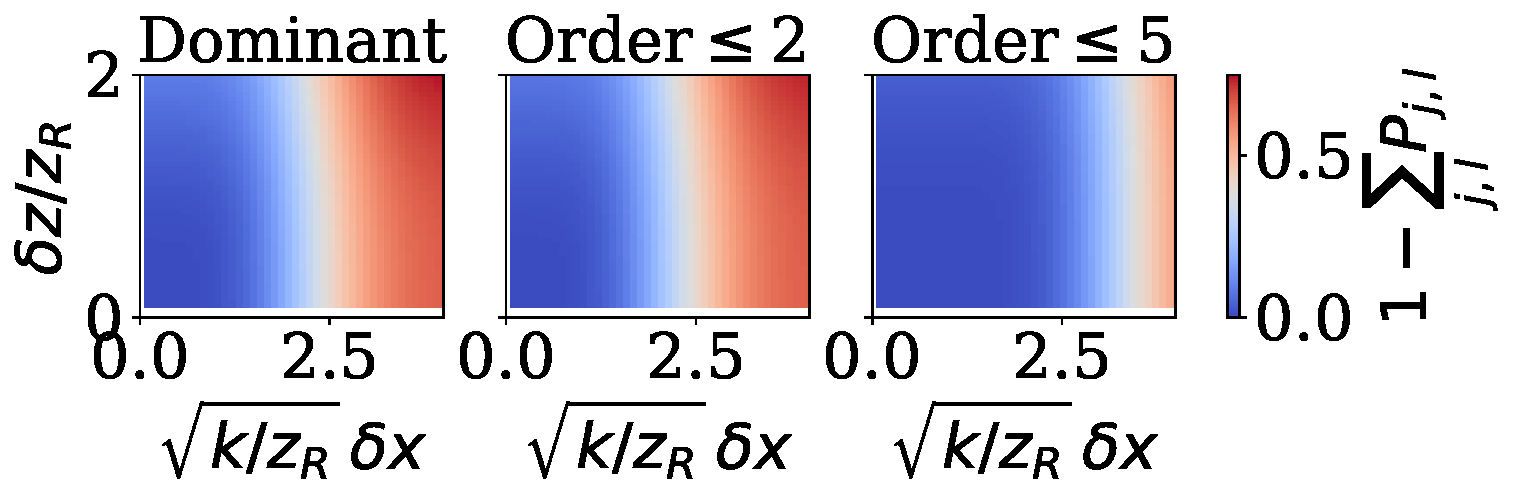
\includegraphics[width=\textwidth]{leaked_fraction_heatmap.pdf}
\caption{Leaked fraction of collected light not routed into a resolved mode $L=1-\sum_{(j,l)\in\mathcal{M}}P_{j,l}$ over the crack width $\delta x$ and depth $\delta z$. The leaked fraction is fourth-order small in the sub-Rayleigh regime and is reduced further by resolving more modes. \textbf{Left:} Four dominant modes [(0,0), (1,0), (2,0), (0,2)] (``Dominant''). \textbf{Middle/Right:} increasing measurement channel to capture modes up to mode-order ($2$, $5$).}
\label{fig:leaked_fraction}
\end{figure*}

\begin{figure*}[h]
\centering
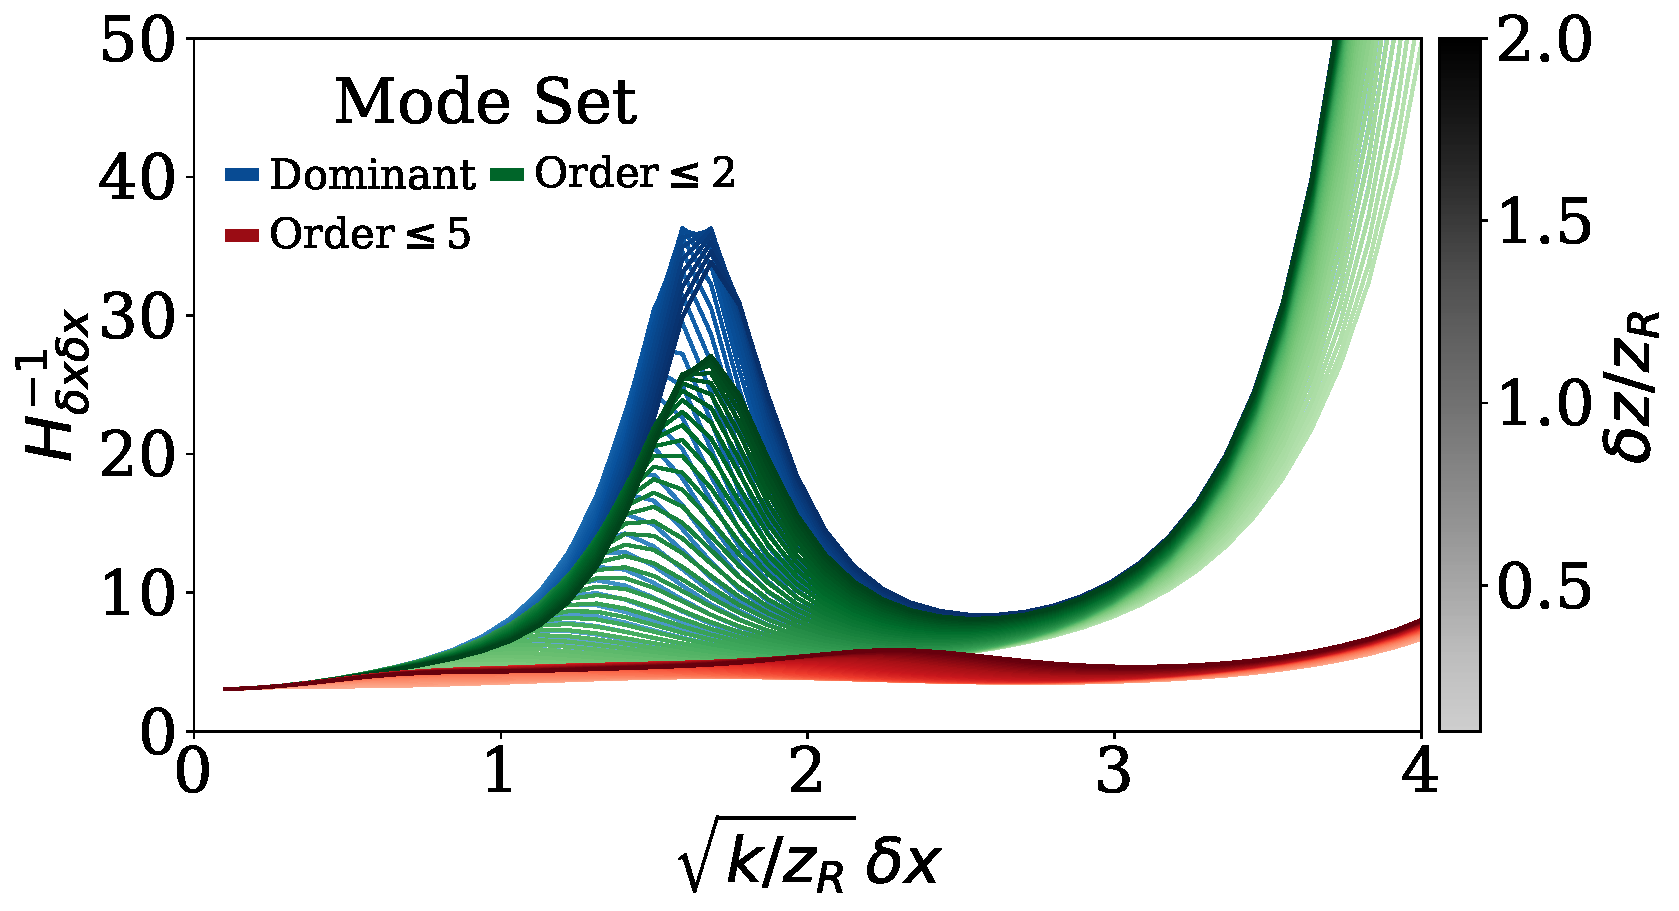
\includegraphics[width=0.45\columnwidth]{crb_convergence_width.pdf}\qquad
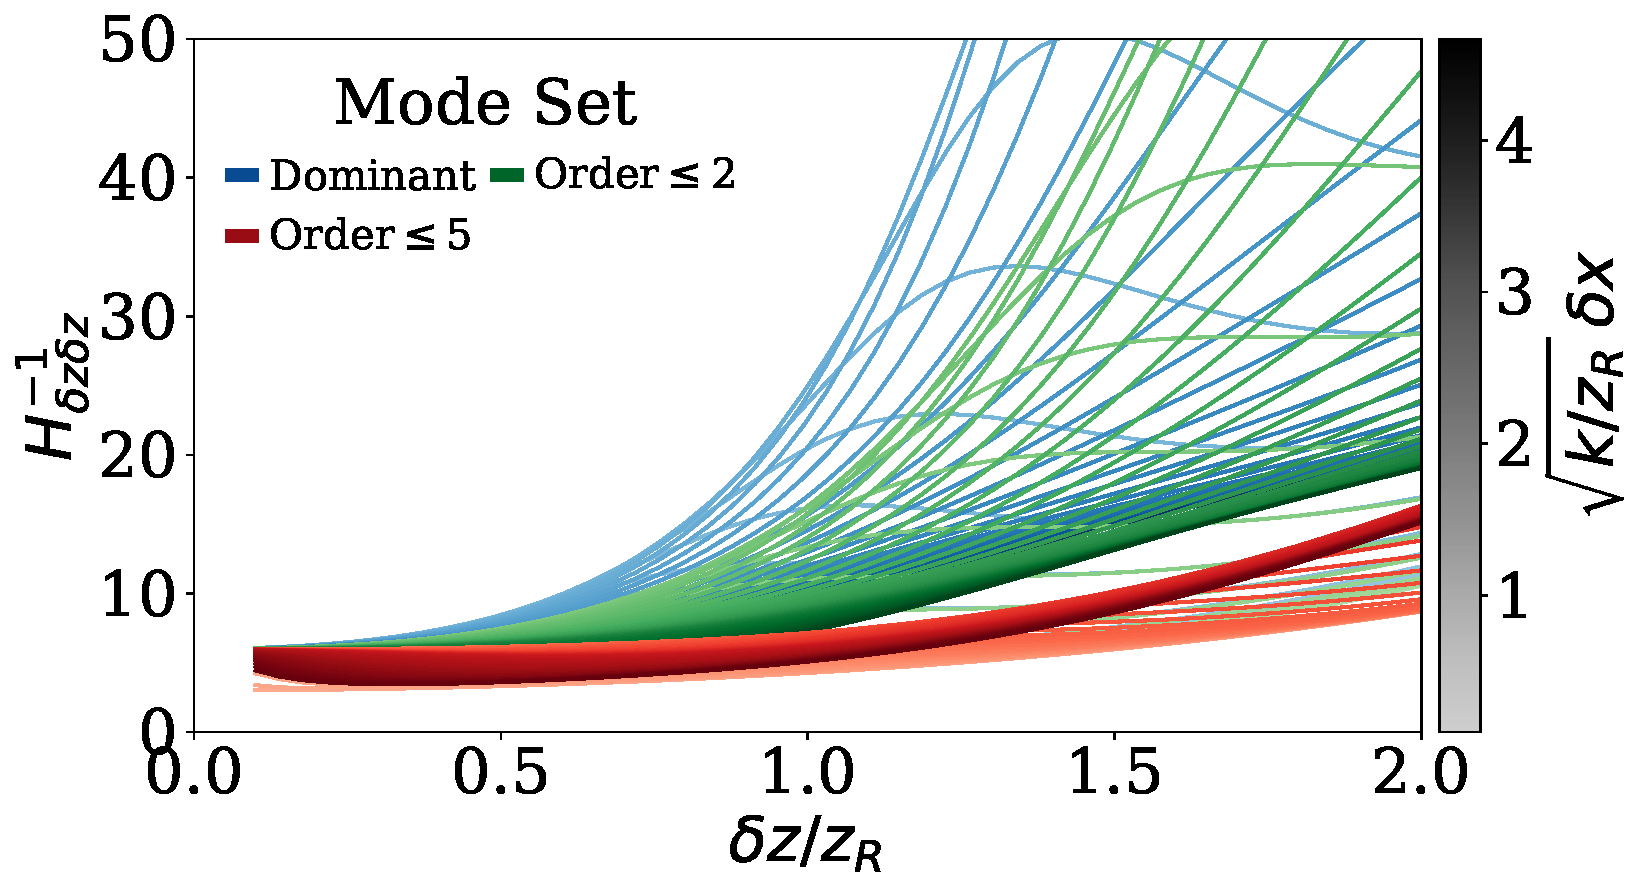
\includegraphics[width=0.45\columnwidth]{crb_convergence_depth.pdf}
\caption{Convergence of the mode-sorting Cram\'er-Rao bound to the quantum limit as the resolved number of modes is increased, for the width $\delta x$ (left) and depth $\delta z$ (right), each including the remainder channel. The minimal four-mode measurement (``Dominant'') already saturates the quantum limit in the sub-Rayleigh regime; resolving additional modes only extends the useful range to larger separations, where direct imaging already approaches the quantum limit, confirming the sufficiency of the minimal bank.}
\label{fig:crb_convergence}
\end{figure*}
}


% \section{Impact of Mode-Sorting Imperfections on the Classical Fisher Information\label{app:ms_errors}}
\section{{\color{red}Mode-Sorting Bounds under Experimental Imperfections}\label{app:ms_errors}}
{\color{red}
A realistic mode-sorting measurement is subject to two distinct imperfections, which we treat in turn: (i) imperfect sorting, in which the device leaks amplitude between neighbouring Hermite-Gaussian orders (cross-talk), and (ii) a detector noise floor of $\theta$-independent counts arising from dark counts and background light. The former corrupts the measurement basis itself, whereas the latter adds a noise background to otherwise ideal channels; we show that the mode-sorting advantage survives both.}
\paragraph{{\color{red}(i) Mode cross-talk.}}
{\color{red}
A practical mode sorter does not project onto perfectly resolved Hermite-Gaussian modes. The most common experimental realisation of mode sorting is achieved via Multi-plane light converters. Such devices are known to exhibit finite {\em cross-talk}, in which a small fraction of the light intended for one mode is registered in a mode of neighbouring order~\cite{gessner2020spadeerror,modes,MPLC}. Since this leakage is (to leading order) a {\em nearest-neighbour} effect, we model it as such here.

We incorporate this imperfection at the level of the measurement basis, before computing the detection probabilities, their derivatives, and the Fisher information. Denoting the truncated one-dimensional HG basis by $\{\phi_n\}_{n=0}^{N-1}$, we couple adjacent orders with a lossless beam splitter
\begin{equation}
R_{n,n+1}(\epsilon):\quad
\begin{pmatrix}\phi_n\\ \phi_{n+1}\end{pmatrix}
\longmapsto
\begin{pmatrix}\cos\epsilon & -\sin\epsilon\\ \sin\epsilon & \phantom{-}\cos\epsilon\end{pmatrix}
\begin{pmatrix}\phi_n\\ \phi_{n+1}\end{pmatrix},
\end{equation}
and apply the chain $U(\epsilon)=R_{N-2,N-1}(\epsilon)\cdots R_{1,2}(\epsilon)\,R_{0,1}(\epsilon)$ to the $x$- and $y$-mode indices independently, so that the two-dimensional measurement modes are transformed by $U(\epsilon)\otimes U(\epsilon)$. Crucially, $U(\epsilon)$ is orthogonal, $U^{\!\top} U=\openone$, so the mixed modes remain orthonormal. As for the ideal measurement, we then resolve only the same information-bearing modes $(0,0)$, $(1,0)$, $(2,0)$, $(0,2)$, which now include cross-talk, and collect all unresolved light, including the amplitude leaked into neighbouring orders, in the remainder channel (Appendix~\ref{app:remainder}). The measurement therefore remains the same complete POVM used throughout, and the derivations in Appendices~\ref{app:ms_incoherent} and~\ref{app:remainder} carry over verbatim.

We quantify the cross-talk strength in decibels through the amplitude transferred across a single adjacent coupling,
\begin{equation}
\mathrm{xt}\;[\mathrm{dB}]\equiv 20\log_{10}(\sin\epsilon),
\end{equation}
so that a fraction $\sin^2\epsilon=10^{\,\mathrm{xt}/10}$ of the power leaks across each nearest-neighbour pair (for instance $-20$~dB corresponds to $\sin\epsilon=0.1$, i.e.\ $1\%$ leaked power per coupling). In the sequential construction above, an interior mode of order $n$ participates in two rotations, $R_{n-1,n}$ and $R_{n,n+1}$, and therefore leaks roughly twice as much power as a boundary mode. The quoted dB should thus be read as the strength of an individual adjacent coupling rather than as a uniform per-mode leakage.}

\begin{figure*}[h]
\centering
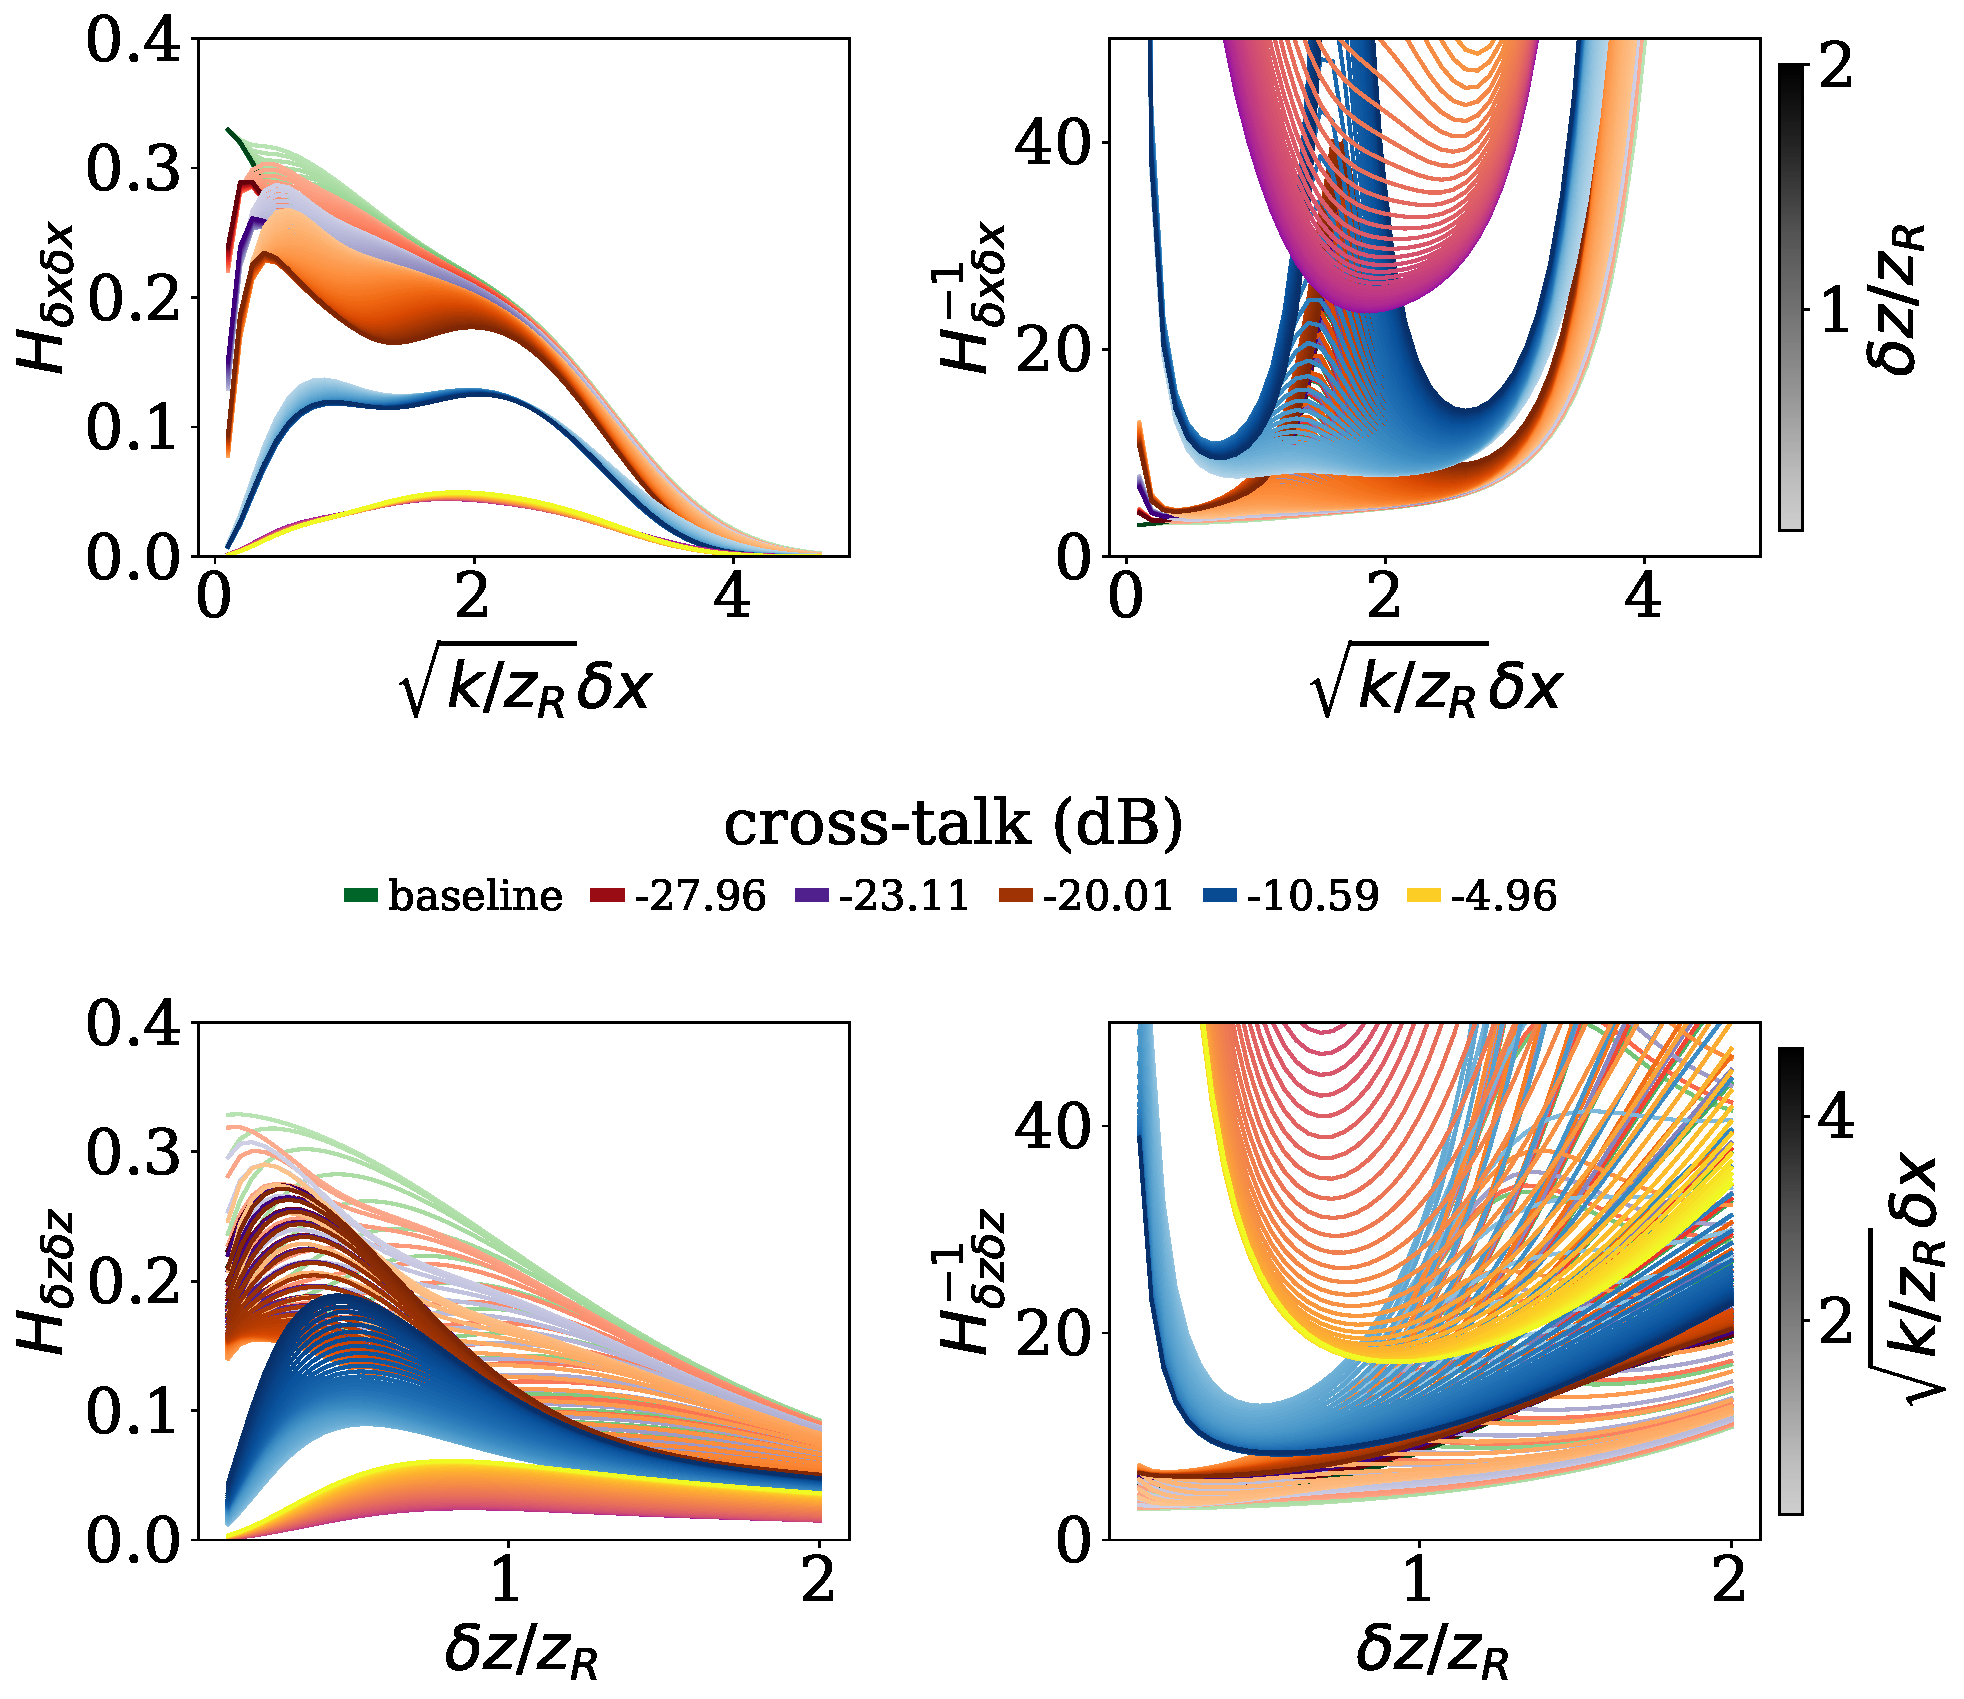
\includegraphics[width=0.9\columnwidth]{combined_fi_crb_mixing.pdf}
\caption{{\color{red}Effect of nearest-neighbour mode cross-talk on the classical Fisher information of the Hermite-Gaussian mode-sorting measurement, for the incoherent three-source crack model. Left column: Fisher information; right column: the associated Cram\'er-Rao bound. Top row: estimation of the width parameter $\delta x$ for various depths $\delta z$; bottom row: depth parameter $\delta z$ for various widths $\delta x$. For each colour family the gradient encodes the value of the secondary parameter (grayscale colorbar to the right). Curve colour encodes the cross-talk strength $20\log_{10}(\sin\epsilon)$ in dB (legend), from the ideal baseline ($\epsilon=0$) up to $\approx-5$~dB. Increasing cross-talk lowers the Fisher information and raises the Cram\'er-Rao bound, but the degradation remains moderate up to $-20$~dB.}}
\label{fig:ms_errors}
\end{figure*}

{\color{red}
Figure~\ref{fig:ms_errors} shows the effect of cross-talk on the Fisher information (left column) and the corresponding Cram\'er-Rao bound (right column) for the width parameter $\delta x$ (top row) and the depth parameter $\delta z$ (bottom row), as the cross-talk is swept from the ideal baseline (no cross-talk) up to $\approx-5$~dB. As anticipated, stronger cross-talk degrades the Fisher information and inflates the Cram\'er-Rao bound. The degradation is pronounced precisely because the parameter information is concentrated in a small number of modes: the width $\delta x$ is carried almost entirely by the first-order mode $(1,0)$, while the depth $\delta z$ is carried by the second-order modes $(0,2)$ and $(2,0)$ associated with axial defocus (cf.\ Fig.~\ref{fig:supp4figs}). Mixing rotates amplitude out of these information-bearing modes into neighbouring orders, which are unresolved and merged into the remainder channel where only their aggregate is retained, so the measurement loses sensitivity faster than a uniform-loss model would predict. The effect is sharpest where essentially a single mode is responsible for estimating a given parameter.

However, for cross-talk up to $-20$~dB, which is experimentally attainable~\cite{bearne2026ModeSorting,kupianskyi2023MS,Fontaine2017DesignOH}, the Fisher information is reduced but does not collapse, and throughout the sub-Rayleigh regime it remains above the direct-imaging benchmark established in Fig.~\ref{fig:supp4figs}; direct imaging becomes competitive only as the Rayleigh length is approached, where it is preferable in any case. The loss relative to the ideal sorter is mild over most of this range (of order $15$--$25\%$), becoming pronounced only in the deepest sub-Rayleigh limit of the width estimation, where the nearly empty $(1,0)$ mode is swamped by leakage from the bright fundamental mode $(0,0)$; even there, mode sorting still sits well above direct imaging. Mode sorting therefore retains its advantage over conventional direct imaging under realistic, imperfect sorting; only with larger cross-talk does this advantage erode.}

\begin{figure*}[h]
\centering
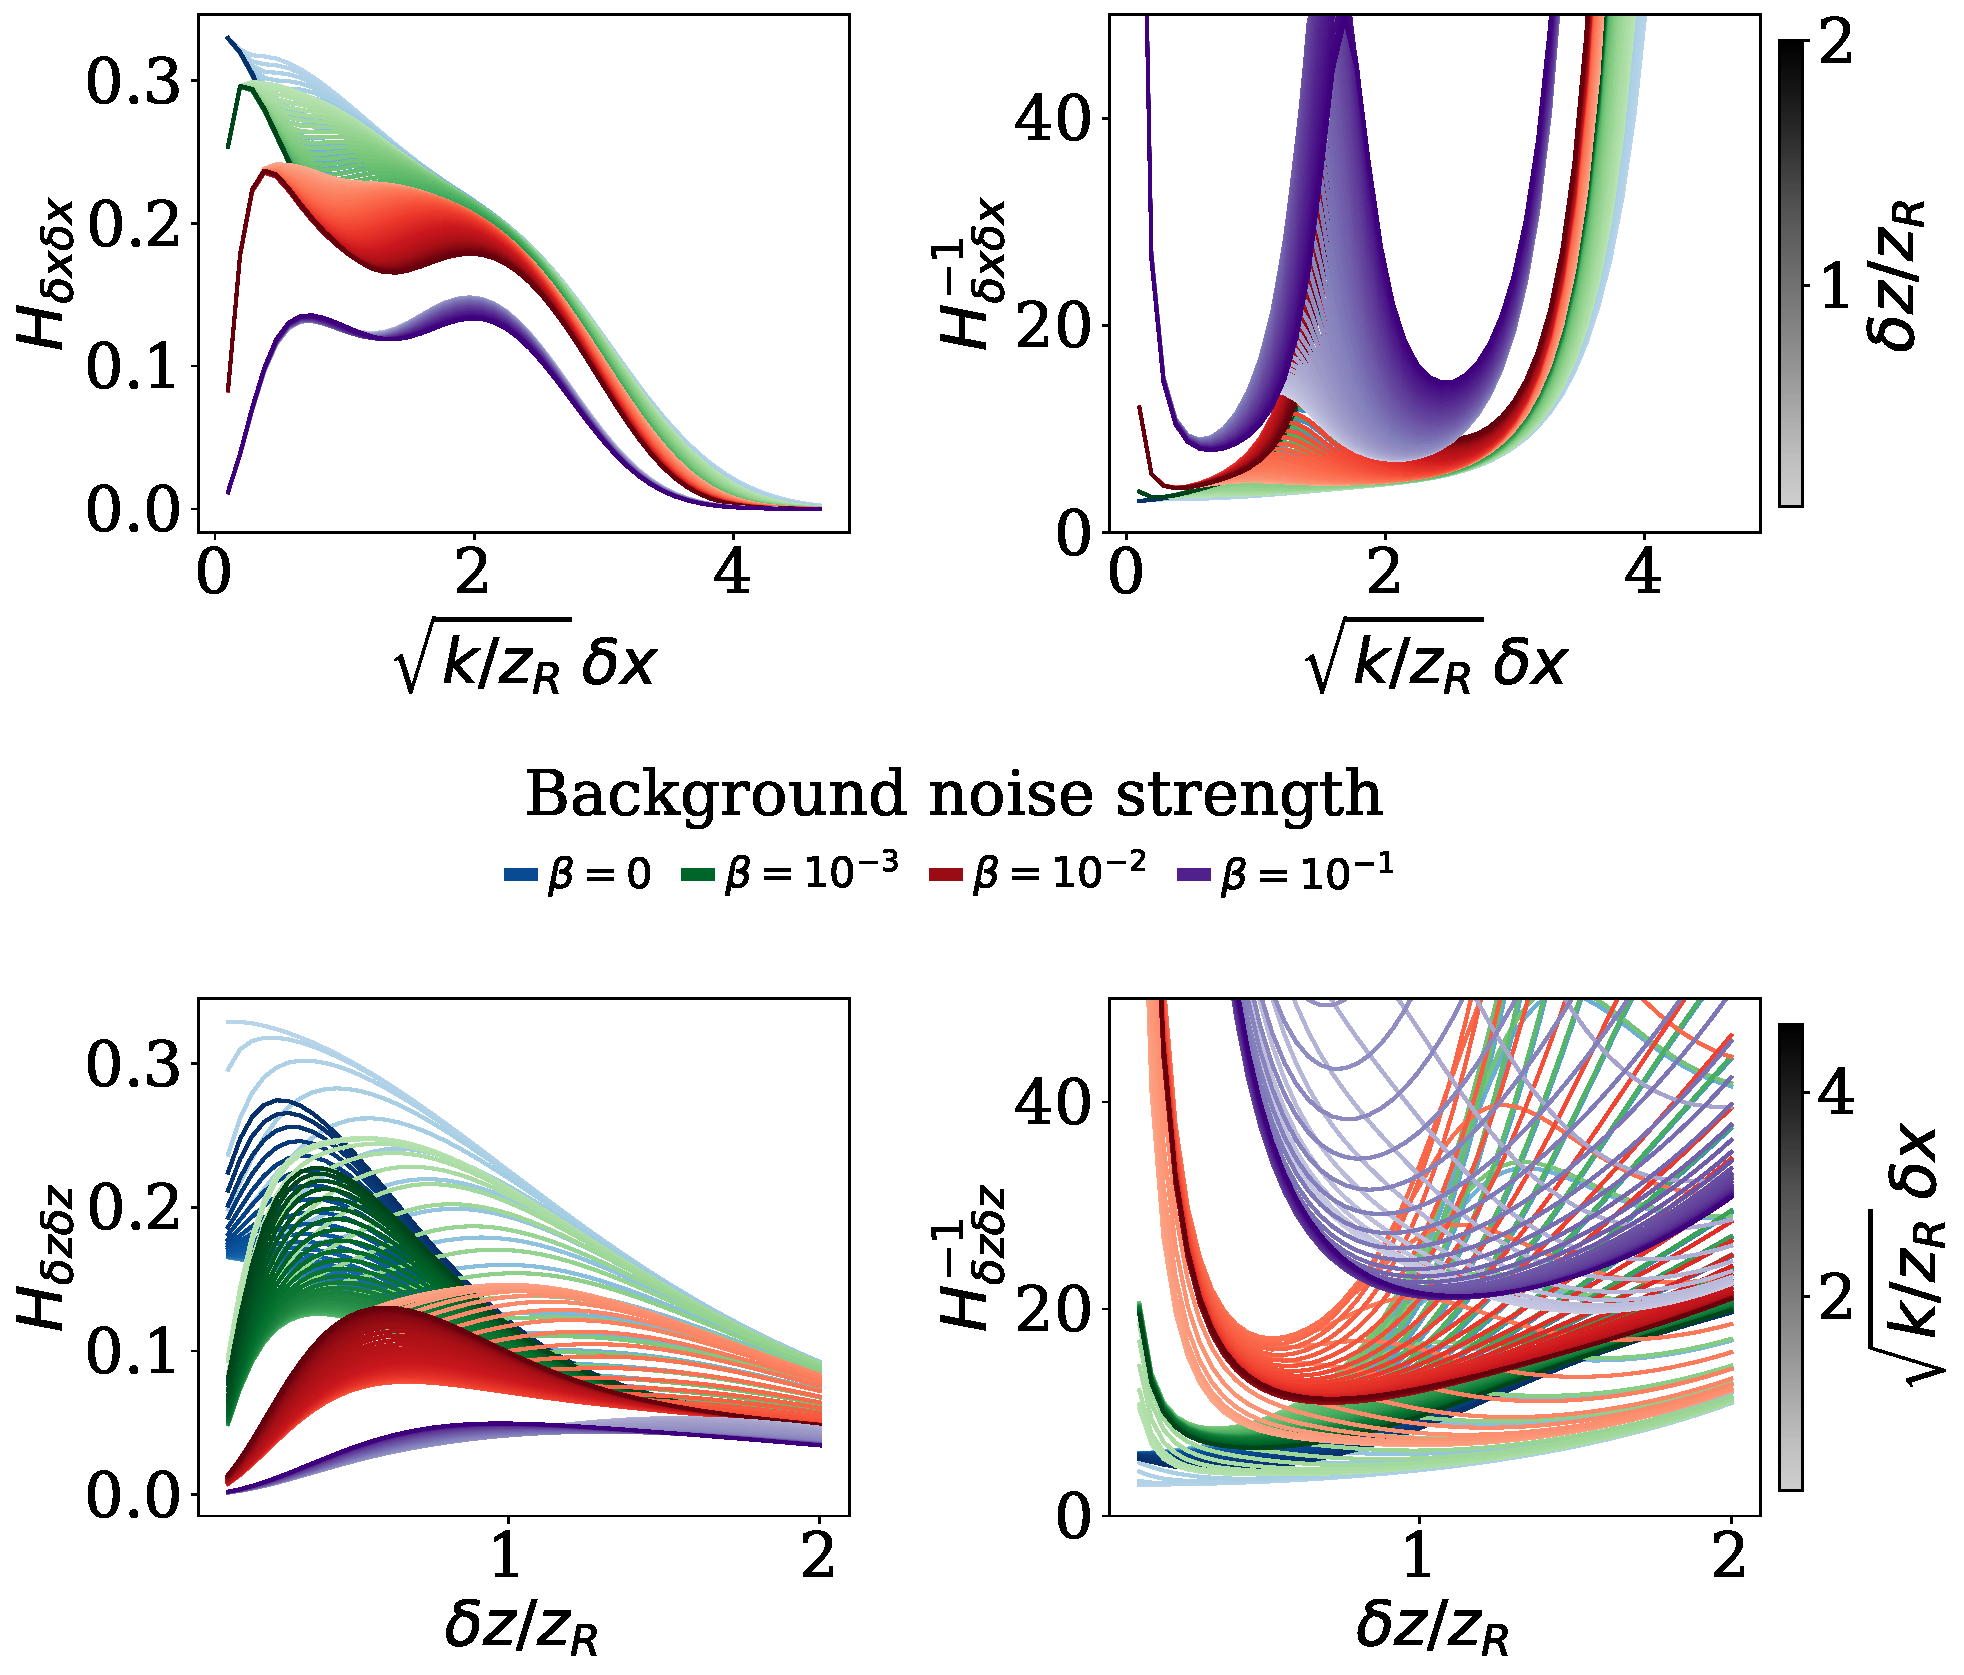
\includegraphics[width=0.9\columnwidth]{combined_fi_crb_noise.pdf}
\caption{{\color{red}Effect of an additive detector noise floor (dark counts and background light) on the classical Fisher information of the Hermite-Gaussian mode-sorting measurement: left column, Fisher information; right column, the associated Cram\'er-Rao bound; top row, the width parameter $\delta x$ for various depths $\delta z$; bottom row, the depth parameter $\delta z$ for various widths $\delta x$. For each colour family the gradient encodes the value of the secondary parameter (grayscale colorbar to the right). Curve colour encodes the background-to-signal ratio $\beta=b_j/\tau$ (legend), from the ideal baseline ($\beta=0$) up to $\beta=10^{-1}$. The floor enters the Fisher-information denominator and suppresses low-occupancy channels first, so the depth bound is inflated faster than the width bound.}}
\label{fig:ms_noise}
\end{figure*}

\paragraph{{\color{red}(ii) Detector noise floor.}}
{\color{red}
The Poissonian model in Eq.~\eqref{eq:FI_MS} already captures photon shot noise. A uniform optical or detector inefficiency $\eta$ simply thins the Poisson process, $\tau\to\eta\tau$, rescaling every channel mean by the same factor; it scales the overall Fisher information but leaves the mode-sorting-versus-direct-imaging comparison unchanged, since both schemes are rescaled equally. A genuine detector noise floor is qualitatively different: dark counts and background light add a $\theta$-independent count floor $b_j$ to each channel, so the mean registered power becomes $\lambda_j=\tau P_j(\theta)+b_j$. Because $b_j$ is independent of $\theta$ we have $\partial_a\lambda_j=\tau\,\partial_a P_j$, and the Fisher information Eq.~\eqref{eq:FI_MS} generalises to
\begin{equation}
({J_\Pi})_{a,b}=\tau^2\sum_j^M\frac{1}{\tau P_j(\theta)+b_j}\pdv{P_j(\theta)}{\theta_a}\pdv{P_j(\theta)}{\theta_b}.
\label{eq:FI_MS_noise}
\end{equation}
We parametrise the floor by the background-to-signal ratio $\beta_j\equiv b_j/\tau$ and take it uniform across the measurement channels, $\beta_j=\beta$, at fixed photon budget $\tau$.}

{\color{red}
Figure~\ref{fig:ms_noise} shows that the background noise lowers the Fisher information, with the depth estimation degrading faster than width. This follows directly from the denominator of Eq.~\eqref{eq:FI_MS_noise}, in which a count floor preferentially suppresses the channels of small occupancy $P_j$ that carry the sub-Rayleigh parameter information. As established above (cf.\ Fig.~\ref{fig:supp4figs}), the width is carried by the first-order mode $(1,0)$ while the depth is carried by the fainter second-order modes $(2,0)$ and $(0,2)$. The degradation nevertheless remains moderate for background-to-signal ratios up to the percent level, becoming severe only once $\beta$ is comparable to the occupancy of these information-bearing modes.}

\section{{\color{red}Robustness to unequal source brightness}\label{app:unequal_intensities}}
{\color{red}
Throughout the main text we assumed equal source intensities $I_v=1/V$ [Eq.~\eqref{eq:incoherent_ensemble}]. Here we relax that assumption and assume \emph{known but unequal} brightness. The imbalance does not change \emph{how well} mode sorting attains the quantum limit, it only \emph{reallocates} a fixed photon budget between the crack-width and crack-depth parameters.

Exploiting the left--right symmetry of the three-source model, we parametrise the imbalance by a single \emph{contrast} ratio
\begin{equation}
r_c \equiv \frac{I_{\mathrm{mid}}}{I_{\mathrm{out}}},
\end{equation}
the brightness of the central (depth, axial) source relative to each of the two transverse (width, planar) sources, at fixed total budget $\sum_v I_v = 1$, so that $I_{\mathrm{mid}}=r_c/(r_c+2)$ and $I_{\mathrm{out}}=1/(r_c+2)$. Here $r_c>1$ brightens the axial source at the expense of the planar pair, $r_c<1$ does the reverse, and $r_c=1$ recovers the equal-brightness model. The closed-form QFIM of Appendix~\ref{app:qfi_derivation} and the mode-sorting Fisher information of Appendix~\ref{app:ms_incoherent} carry over with $1/V\to I_v$ threaded through the density matrix $R_\Delta=\mathrm{diag}(I_1,\dots,I_V)$ and the detection probabilities $P_{j,l}=\sum_v I_v\,\abs{\braket{\phi_{j,l}}{\psi_v}}^2$; both remain in closed form.

\paragraph{{\color{red}(i) Information versus contrast.}}
Figure~\ref{fig:contrast_fi_crb} shows the quantum and mode-sorting Fisher information, and the associated Cram\'er-Rao bounds, as a function of $r_c$ for three representative $(\delta x,\delta z)$ pairs in the sub-Rayleigh regime. Both estimators vary smoothly with brightness and, crucially, track one another: raising $r_c$ increases the depth information and decreases the width information, and vice versa.

\begin{figure*}[h]
\centering
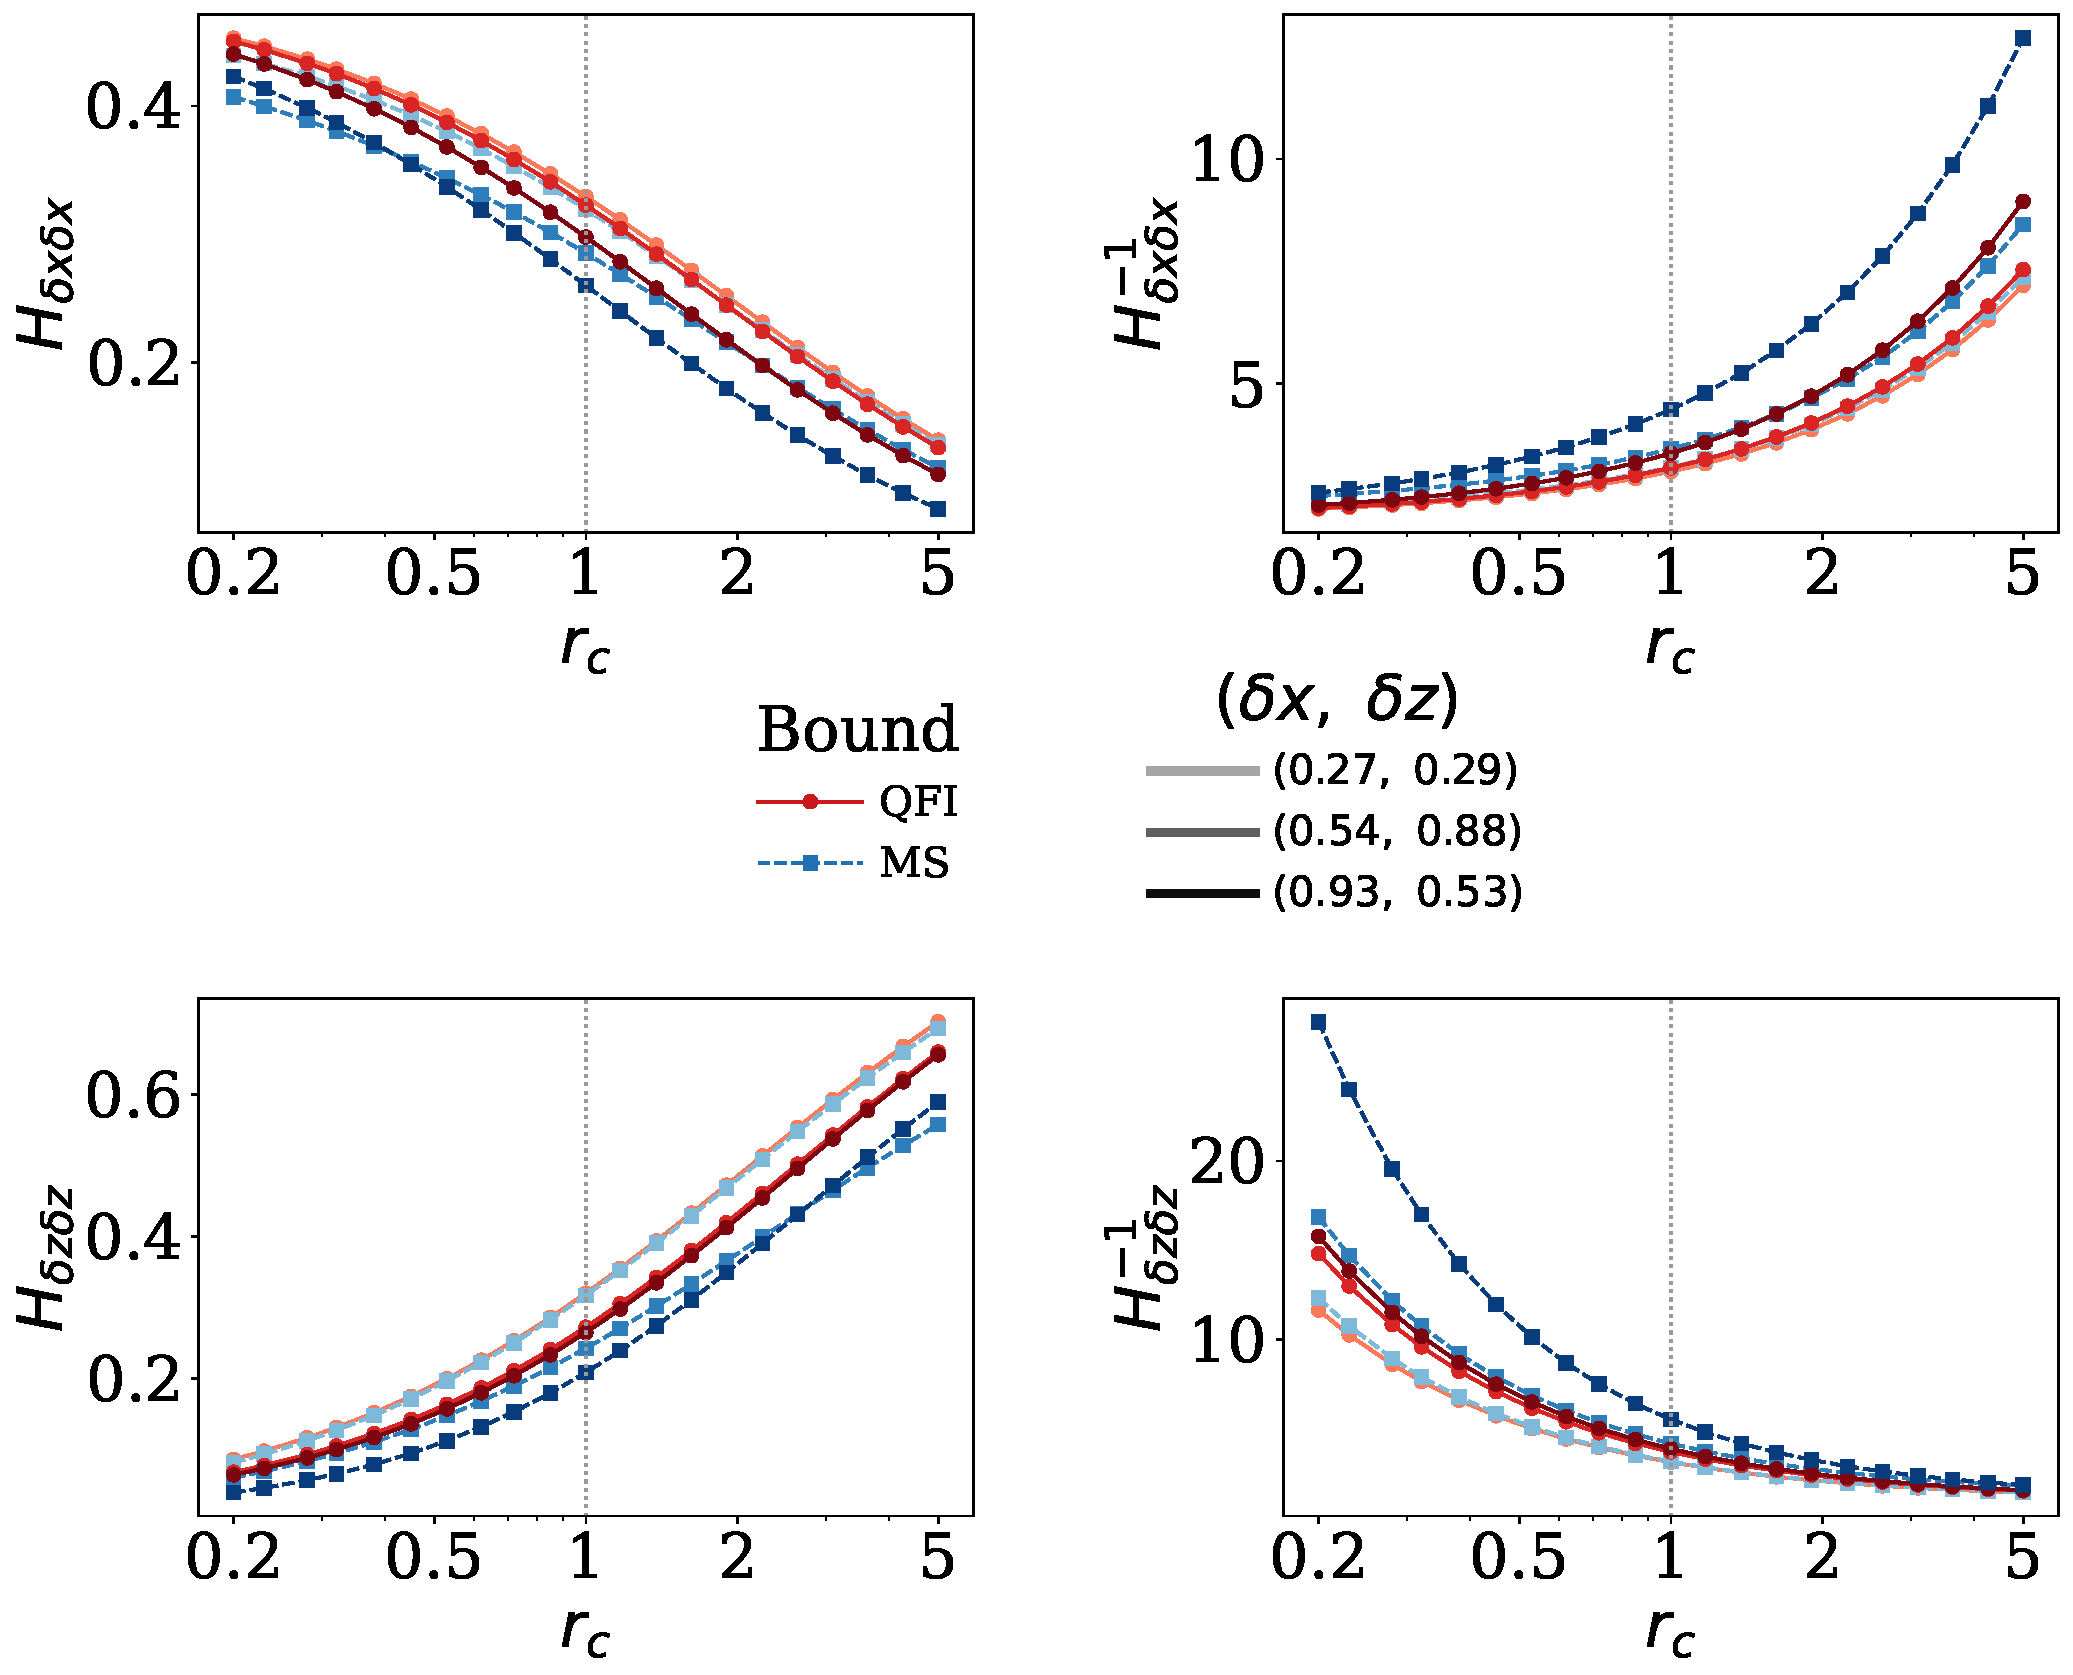
\includegraphics[width=0.85\textwidth]{fi_crb_vs_contrast.pdf}
\caption{{\color{red}Quantum [Red] and MS [Blue] Fisher information [Left], and the associated Cram\'er-Rao bounds [Right], versus the brightness contrast $r_c=I_{\mathrm{mid}}/I_{\mathrm{out}}$ for three different crack geometries. The dotted vertical line marks equal brightness ($r_c=1$). Both estimators vary smoothly with contrast and track one another; the asymmetry about $r_c=1$ reflects the nonlinear weight map $I(r_c)=r_c/(r_c+2)$.}}
\label{fig:contrast_fi_crb}
\end{figure*}


\paragraph{{\color{red}(ii) The contrast dependence is (almost) only photon reallocation.}}
To separate genuine structural effects from the trivial redistribution of photons, Fig.~\ref{fig:contrast_realloc} normalises each bound by its equal-brightness value. Both the quantum and MS curves lie close to the pure photon reallocation (dashed line) across the full range, confirming that the contrast dependence is dominated by the fixed budget moving between sources; the small residual departures are the genuine overlap-induced structural effect and are smallest in the sub-Rayleigh regime.

\begin{figure*}[h]
\centering
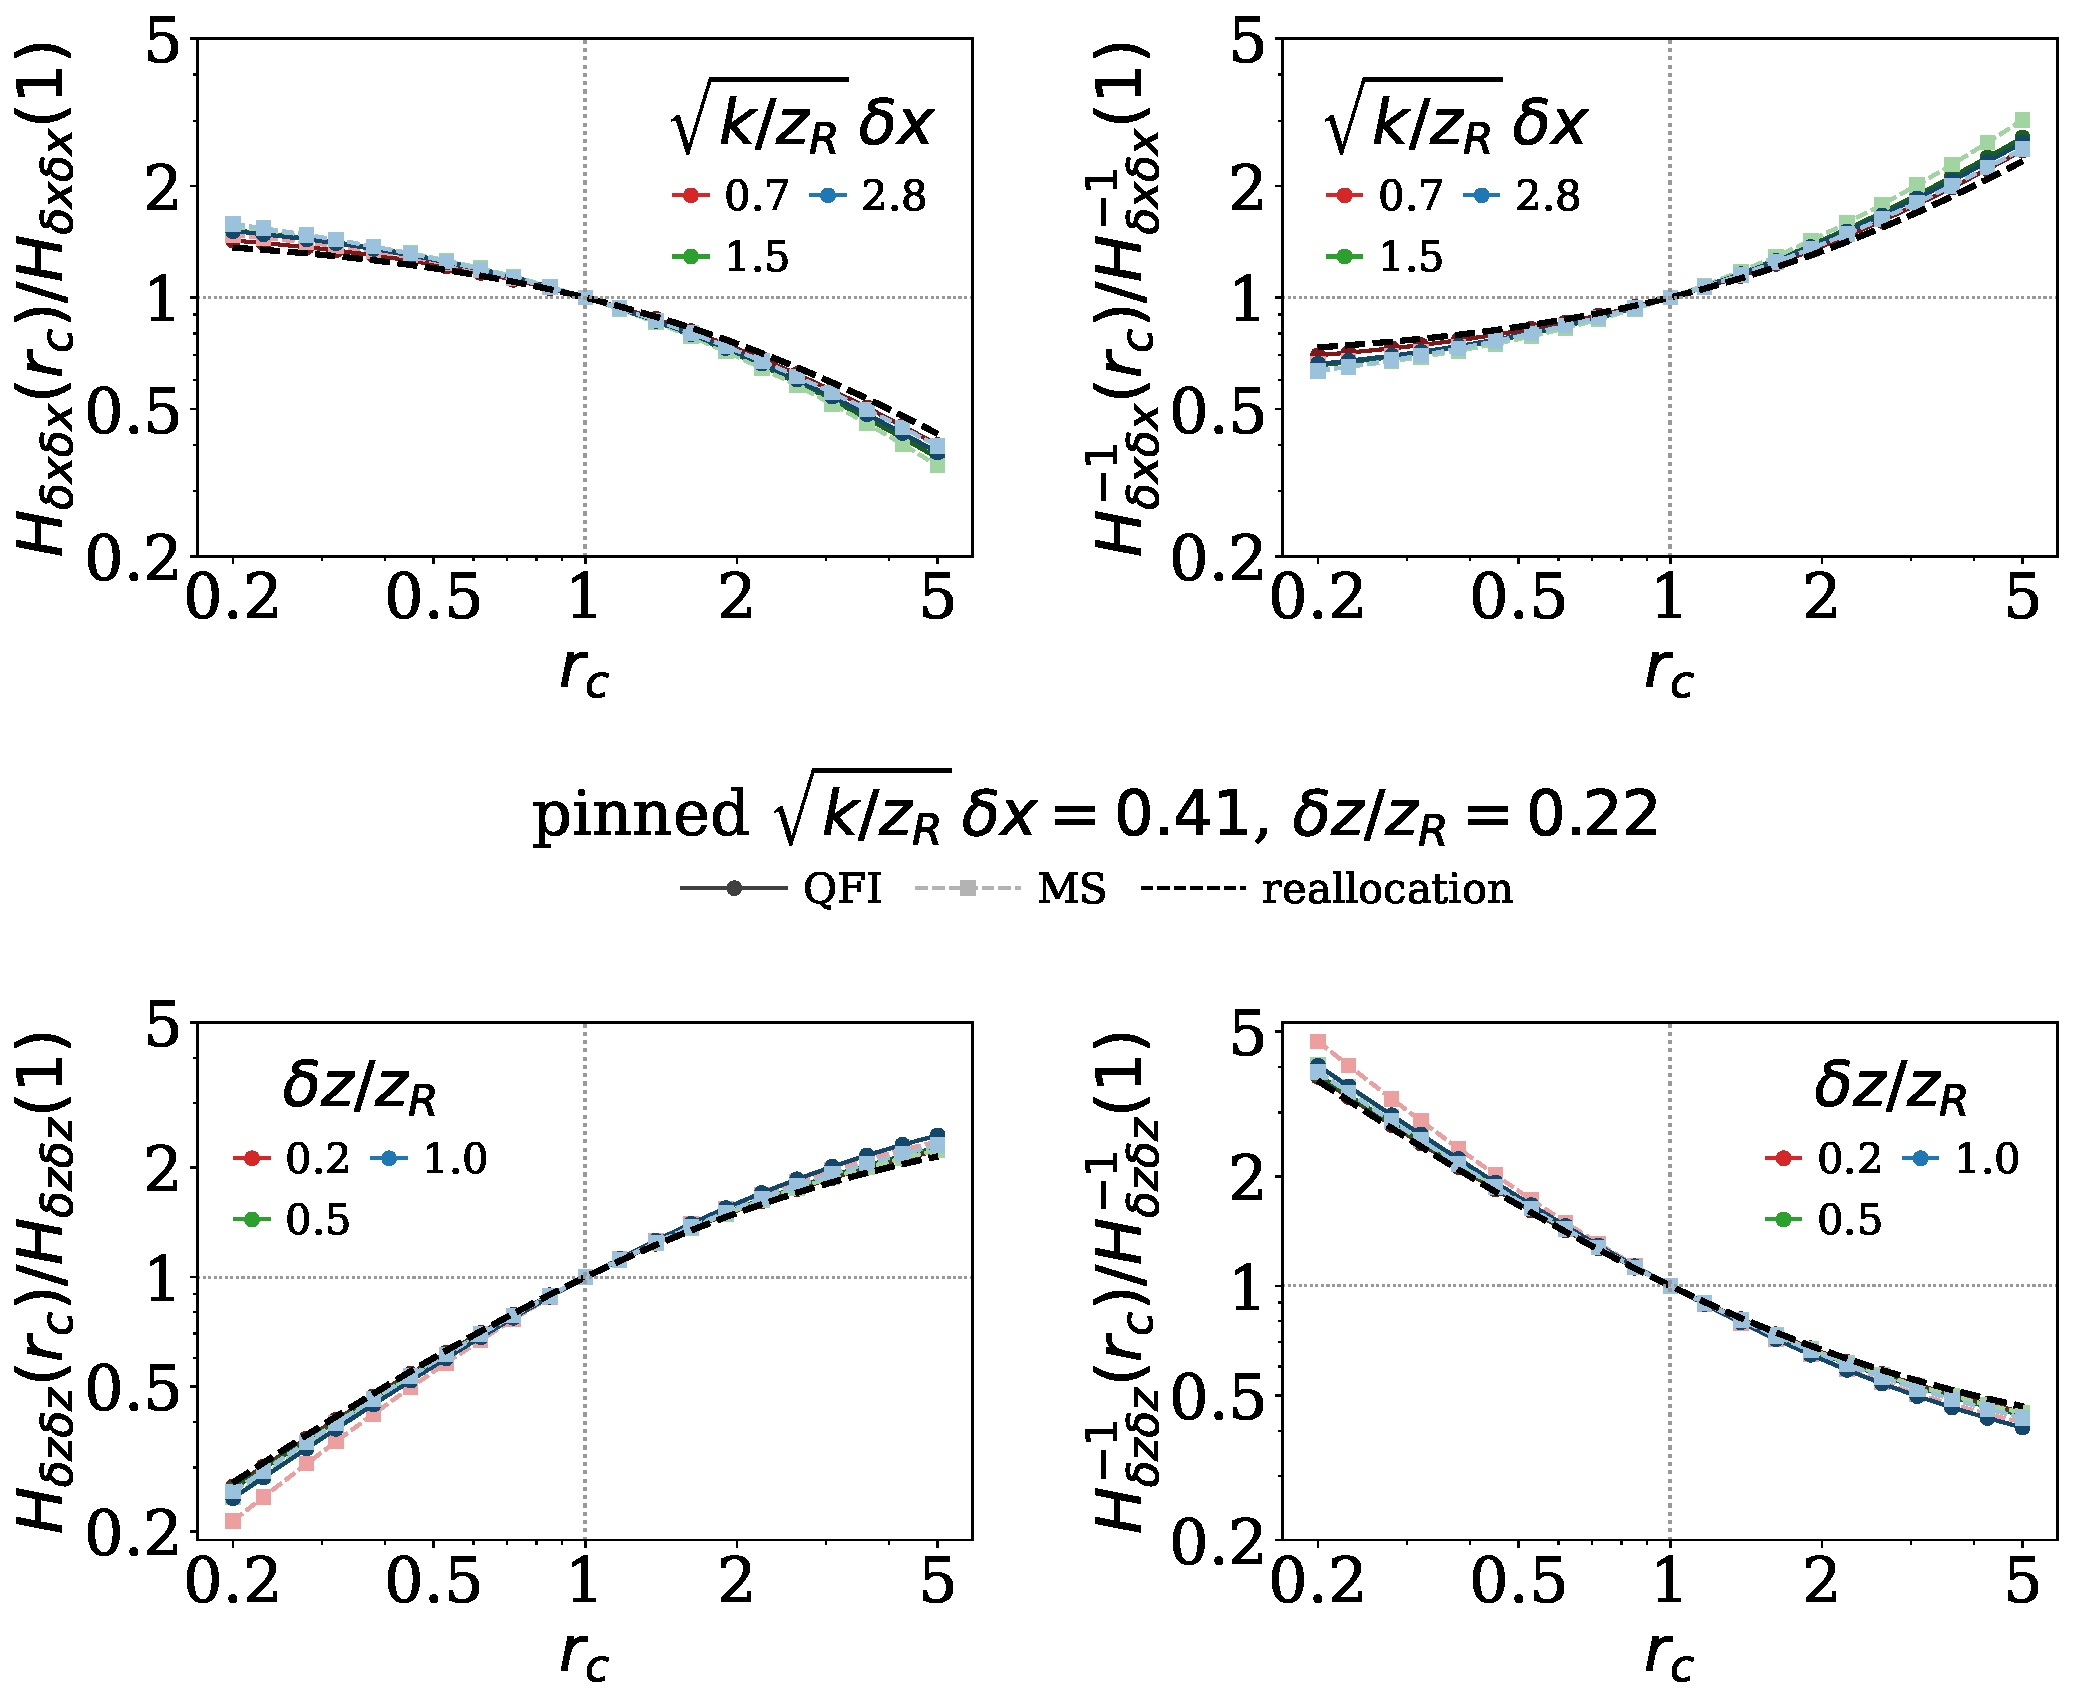
\includegraphics[width=0.85\textwidth]{contrast_reallocation_collapse.pdf}
\caption{{\color{red}Normalised collapse onto the pure-reallocation prediction. Each bound is divided by its equal-brightness ($r_c=1$) value and plotted against contrast (log--log). The dashed black line is the estimator-independent pure-reallocation prediction. Within each panel the swept separation is colour coded (dark = QFI, light = MS) and the orthogonal coordinate is pinned sub-Rayleigh. Curves lying on the dashed line are explained entirely by the photon budget; departures are the genuine structural (overlap) effect.}}
\label{fig:contrast_realloc}
\end{figure*}

\paragraph{{\color{red}(iii) The mode-sorting efficiency is invariant.}}
The decisive quantity for our claim is the efficiency with which mode sorting realises the quantum limit. Figure~\ref{fig:contrast_efficiency} plots the quantum Cram\'er-Rao saturation $H^{-1}/J^{-1}$ as the ratio of the mode-sorting and quantum Cram\'er-Rao bounds against contrast. In the sub-Rayleigh regime the efficiency is flat and close to unity over the entire contrast range, for both width and depth. Brightness imbalance therefore moves information between the two parameters without changing how faithfully mode sorting captures it.


\begin{figure*}[h]
\centering
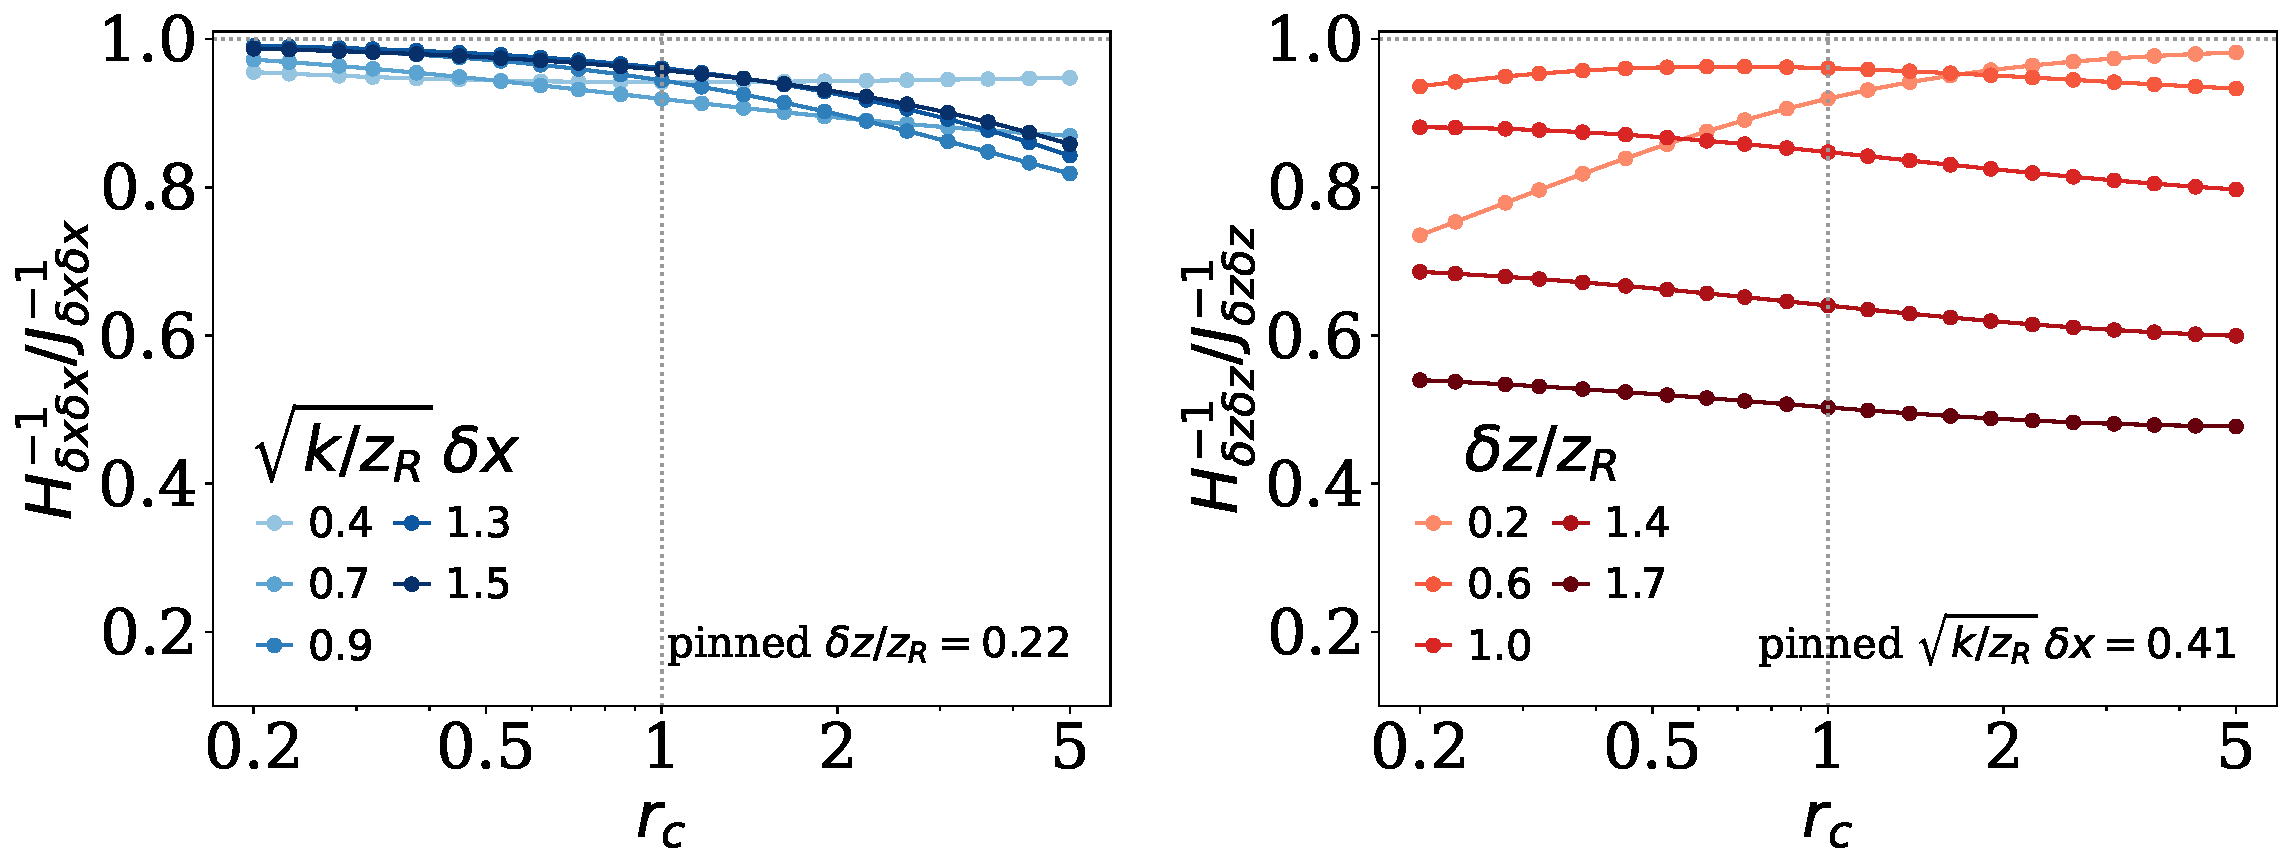
\includegraphics[width=0.9\textwidth]{ms_efficiency_vs_contrast.pdf}
\caption{{\color{red}Mode-sorting efficiency $H^{-1}/J^{-1}$ (ratio of the quantum and mode-sorting Cram\'er-Rao bounds) versus contrast, for the width (left) and depth (right) parameters. Each curve is a fixed separation (light to dark; blue for width, red for depth), with the orthogonal coordinate pinned sub-Rayleigh as noted in each panel. The efficiency stays flat and close to the quantum-optimal value (unity, dotted) across the contrast range in the sub-Rayleigh regime.}}
\label{fig:contrast_efficiency}
\end{figure*}

\paragraph{{\color{red}(iv) The width--depth information exchange.}}
Figure~\ref{fig:contrast_transfer} makes the reallocation explicit. The left panel plots the width information $H_{\delta x\delta x}$ against the depth information $H_{\delta z\delta z}$ as the contrast is swept: as brightness shifts from the planar (width) sources toward the axial (depth) source the locus moves up and to the left, depth information being gained exactly as width information is lost. The right panel shows the same exchange for the associated Cram\'er-Rao bounds, $H^{-1}_{\delta x\delta x}$ against $H^{-1}_{\delta z\delta z}$ (the inverse Fisher information); because the bound is a cost rather than a resource, the trade-off curve is the mirror image and runs in the opposite sense. In the information plane the mode-sorting locus (blue) lies just inside the quantum locus (red), whereas in the bound plane it lies just outside; either way the gap is the mode-sorting shortfall, which is negligible deep sub-Rayleigh and widens only as the separations approach the Rayleigh scale, where direct imaging is preferable in any case.

\begin{figure}[h]
\centering
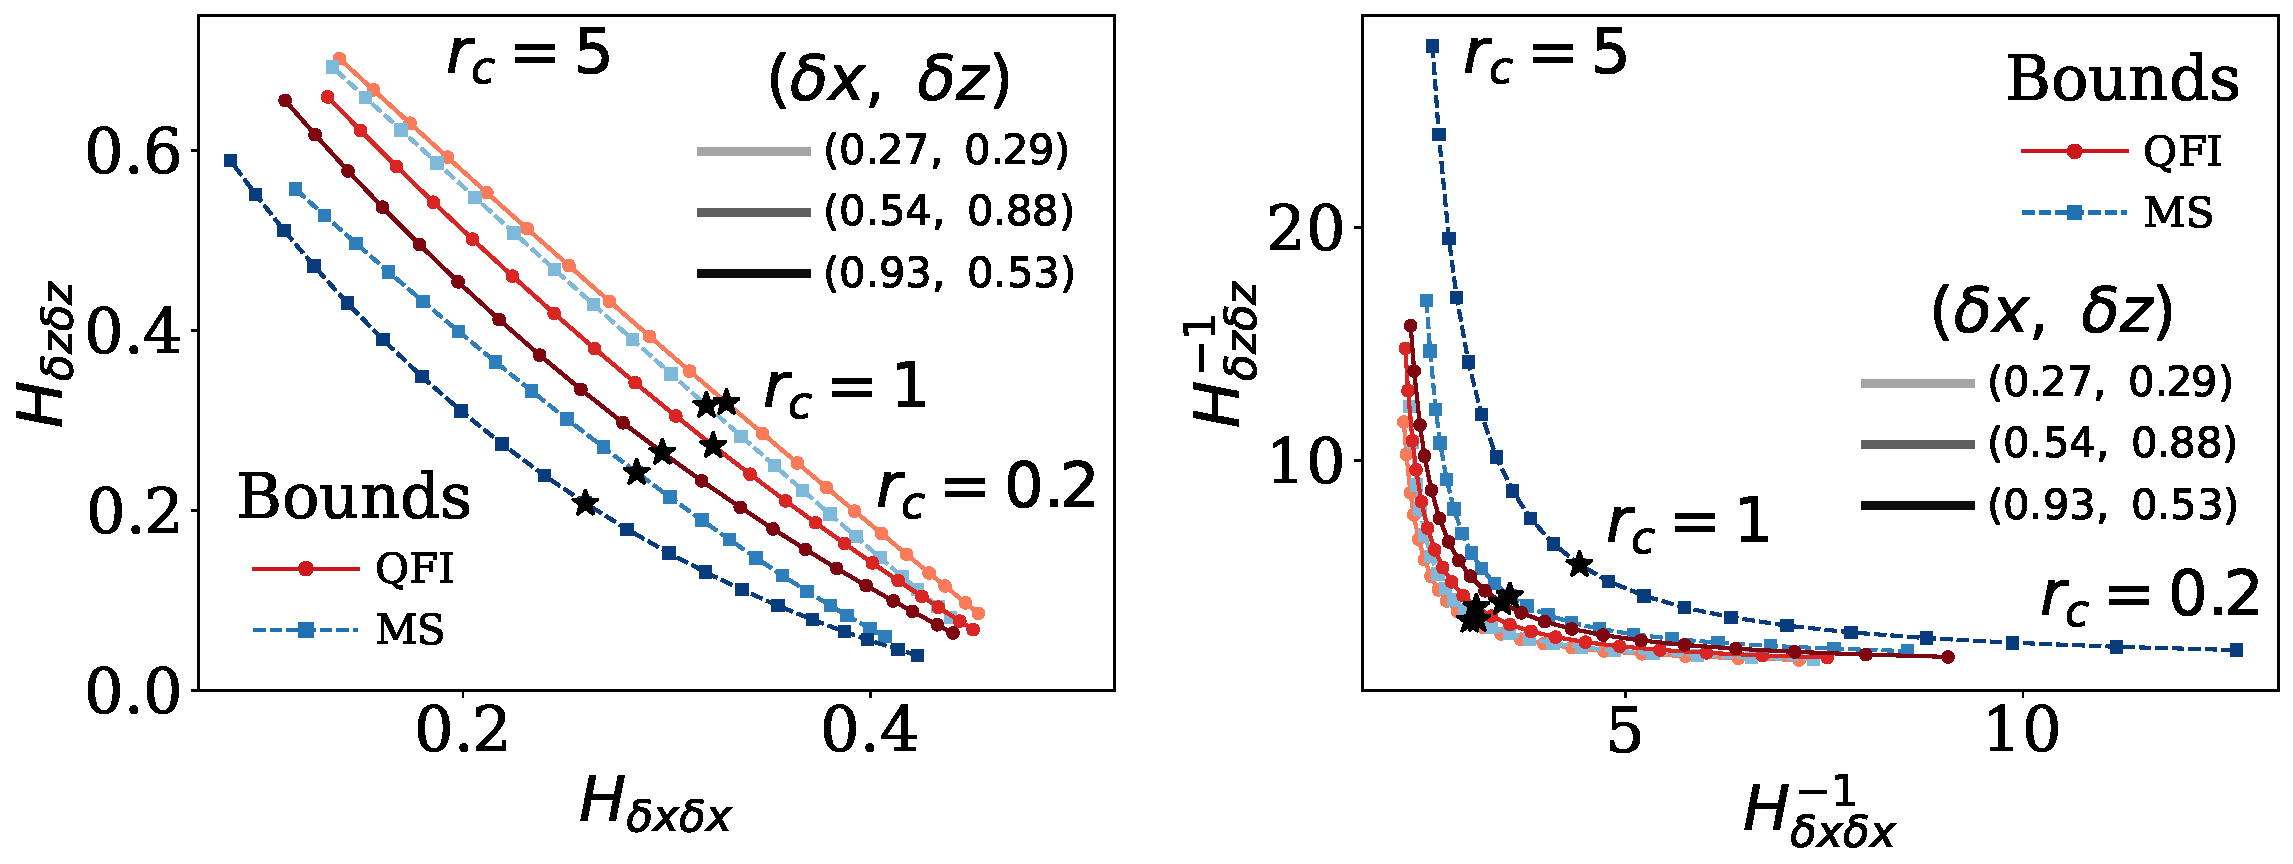
\includegraphics[width=\columnwidth]{contrast_information_transfer.pdf}
\caption{{\color{red}Width--depth information exchange under brightness contrast, for three crack geometries (shade light to dark); the black star marks equal brightness ($r_c=1$). \emph{Left:} the width information $H_{\delta x\delta x}$ against the depth information $H_{\delta z\delta z}$ as the contrast is swept from $r_c=0.2$ (planar bright, bottom-right) to $r_c=5$ (axial bright, top-left). \emph{Right:} the same trade-off for the associated Cram\'er-Rao bounds, $H^{-1}_{\delta x\delta x}$ against $H^{-1}_{\delta z\delta z}$ (inverse Fisher information), which runs in the opposite sense, from $r_c=0.2$ (top-left) to $r_c=5$ (bottom-right). QFI in red, MS in blue. The quantum locus lies inside the MS locus in the information plane and outside it in the bound plane; in both, the mode-sorting shortfall is negligible deep sub-Rayleigh. As brightness shifts toward the axial source, depth information is gained exactly as width information is lost.}}
\label{fig:contrast_transfer}
\end{figure}

\paragraph{{\color{red}Conclusion.}}
Taken together, these results show that relaxing equal brightness does not substantially change the physics of the comparison in the regime of interest. The contrast only reallocates a fixed photon budget between width and depth [Figs.~\ref{fig:contrast_realloc},~\ref{fig:contrast_transfer}], the apparent asymmetry about $r_c=1$ is the nonlinearity of the weight map rather than a structural effect, and the mode-sorting-to-quantum efficiency is essentially invariant sub-Rayleigh [Fig.~\ref{fig:contrast_efficiency}]. Mode sorting therefore remains near-optimal for the simultaneous estimation of crack width and depth, and retains its detection advantage, under unequal source brightness. We may consequently assume equal intensities in the main text without loss of generality.
}


\section{QCB Calculation} \label{app:QCB_calculation}

In this appendix, we describe the numerical methods used to calculate the quantum Chernoff bound and derive an analytical leading-order approximation for the fidelity between the density matrices.

\subsection{Numerical QCB Calculation} \label{app:QCB_calculation_numerical}

To numerically calculate the quantum Chernoff bound, we require an orthonormal basis to represent our density matrices $\rho_0$ and $\rho_1$. This is necessary to calculate the matrix powers $\rho_0^s$ involved in the formula. However, it is worth noting that the QCB is invariant under unitary conjugation, implying that any specific choice of basis should not impact our calculations. Since the point sources are continuous and non-orthogonal, we can use an orthonormal basis that describes the subspace that they span.

To find this subspace basis numerically, we utilise the Gram matrix $G = \braket{\psi_i}{\psi_j}$ of all four point sources $\ket{\psi_L}, \ket{\psi_R}, \ket{\psi_C}$ and $\ket{\psi_Z}$. As all the overlaps between the sources are contained within this matrix, it fully characterises their geometric relationships. By choosing a matrix $A$ such that $G=A^\dagger A$, we can use the columns of $A$ as vector representations of our point sources that have the same geometry. For simplicity, we choose $A = \sqrt{G}$, which exists since the Gram matrix is positive semidefinite. From the vectors we obtain, we can calculate finite dimensional numerical representations of our density matrices for given values of $\delta x$ and $\delta z$.

Having constructed numerical representations of $\rho_0$ and $\rho_1$, we can now calculate their eigenvalues $\lambda_i$, $\mu_j$ and eigenvectors $u_i$, $v_j$ \cite{audenaert2007discriminating}. The QCB is then calculated by minimising the trace
\begin{equation}
    \text{Tr}\left[\rho_0^s \rho_1^{1-s} \right] = \sum_{ij} \lambda_i^s \mu_j^{1-s} \abs{\braket{u_i}{v_j}}^2,
\end{equation}
where $s$ is minimised over the interval $[0,1]$:
\begin{equation}
\xi_Q = -\log \min_{0 \leq s \leq 1} \text{Tr} \left[ \rho_0^s \rho_1^{1-s} \right].
\end{equation}

\subsection{Analytical Fidelity Approximation} \label{app:fidelity_approximation}

For the leading-order expansion of the fidelity
\begin{equation}
F(\rho_0, \rho_1) = \text{Tr}\left[ \sqrt{\sqrt{\rho_0} \rho_1 \sqrt{\rho_0}}\right],
\end{equation}
we use a purification-based method from  \cite{lupo2020quantum}. A density matrix $\rho$ can be represented as ensemble of pure states
\begin{equation}
    \rho = \sum_j p_j \ketbra{\psi_j}{\psi_j}
\end{equation}
where each pure state $\ket{\psi_j}$ is defined using an orthonormal basis $\{\ket{i}\}$
\begin{equation}
\ket{\psi_j} = \sum_i \braket{i}{\psi_j} \ket{i}.
\end{equation}

The purification of $\rho$ is then written as
\begin{equation}
\ket{\Psi} = \sum_{ij} C_{ij} \ket{i} \ket{j},
\end{equation}
where $C_{ij} = \sqrt{p_j} \braket{i}{\psi_j}$ and $\{\ket{j}\}$ is an orthonormal basis representing each source.

For $\rho_0$ and $\rho_1$ we can calculate purifications $\Psi_0$ and $\Psi_1$ with corresponding matrices $C_0$ and $C_1$ respectively. The fidelity is then given by the formula
\begin{equation}
F(\rho_0, \rho_1) = \max_W |\bra{\Psi_0} I \otimes W \ket{\Psi_1}|.
\end{equation}
Using $C_0$ and $C_1$ this can then be reduced to a simple analytical expression
\begin{equation}
\begin{aligned}
F(\rho_0, \rho_1) =& \max_W \left| \sum_{jk} W_{jk} \sum_{i} (C_0)^*_{ij} (C_1)_{ik} \right| \\
=& \max_W \left| \text{Tr}[W^\top M] \right| = \|M\|_1,
\end{aligned}
\end{equation}
where $\|M\|_1 = \text{Tr}[\sqrt{M^\dagger M}]$ is the trace norm and $M = (C_0)^\dagger (C_1) = \sum_i (C_0)^*_{ij} (C_1)_{ik}$.
Through algebraic manipulation, we can express $M$ directly in terms of the overlaps of the ensembles $\rho_0 = \sum_j p_j \ketbra{\psi_j}{\psi_j}$ and $\rho_1  = \sum_k q_k \ketbra{\phi_k}{\phi_k}$
\begin{equation}
\begin{aligned}
M_{jk} =& \sum_i (C_0^*)_{ij} (C_1)_{ik}\\
= & \sum_{i} (\sqrt{p_j}\braket{i}{\psi_j})^*(\sqrt{q_k} \braket{i}{\phi_k})\\
= & \sqrt{p_j q_k} \sum_i \braket{\psi_j}{i} \braket{i}{\phi_k} = \sqrt{p_j q_k} \braket{\psi_j}{\phi_k}.
\end{aligned}
\end{equation}

By demonstrating that $M$ is a weighted overlap matrix, we show that it is also independent of the basis $\{\ket{i}\}$ used to represent each of the pure states $\ket{\psi_j}$ and $\ket{\phi_j}$.
Furthermore, the trace norm $\|M\|_1$ is also independent of the pure state ensemble used to represent the density matrix. This is due to changes in ensembles acting as right-multiplication by a unitary on the individual purification matrix $C' = CU$. Consequently, given a change of ensemble in $\rho_0$ and $\rho_1$ corresponds to $C'_0 = C_0U_0$ and $C'_1 = C_1U_1$, the resulting matrix is then described as  $M' = C_0'^\dagger C'_1 = U_0^\dagger C_0^\dagger C_1 U_1 = U_0^\dagger MU_1$. Since the trace norm is invariant under multiplication from unitaries on either side $\|M'\|_1 = \|U_0^\dagger M U_1 \|_1 = \|M\|_1$, the value of the fidelity is also invariant.

Using these properties, we can create a matrix $M$ using a convenient choice of basis. To do so we first define the following notation for the overlaps of our pure states
\begin{equation}
\begin{aligned}
\alpha =& \braket{\psi_L}{\psi_C} = \braket{\psi_R}{\psi_C} = \exp \left(-\frac{\delta x^2}{16} \right) \\
\beta =& \braket{\psi_L}{\psi_Z} = \braket{\psi_R}{\psi_Z} = \frac{2i}{\delta z + 2i} \exp \left(-\frac{i \delta x^2}{8(\delta z + 2i)} - i k z_R \delta z \right) \\
\gamma =& \braket{\psi_C}{\psi_Z} = \frac{2i}{\delta z + 2i} \exp \left( -i k z_R \delta z \right)
\end{aligned}
\end{equation}
and additionally,
\begin{equation}
\braket{\psi_L}{\psi_R} = \exp \left(-\frac{\delta x^2}{4} \right) = \alpha^4.
\end{equation}
To simplify the matrix $M$, we can recognise that both $\rho_0$ and $\rho_1$ contain the same states $\ket{\psi_L}$ and $\ket{\psi_R}$. Furthermore, since both states have the same overlap with $\ket{\psi_C}$ and $\ket{\psi_Z}$ due to symmetry, we introduce the two parity states
\begin{equation}
\begin{aligned}
\ket{+} =&\frac{\ket{\psi_L} + \ket{\psi_R}}{\sqrt{2 + 2\alpha^4}} \\
\ket{-} =& \frac{\ket{\psi_L} - \ket{\psi_R}}{\sqrt{2 - 2\alpha^4}}.
\end{aligned}
\end{equation}
These provide us with an alternative description of our quantum states
\begin{equation}
\begin{aligned}
\rho_0 =& \frac{(1+\alpha^4)\ketbra{+}{+} + (1-\alpha^4)\ketbra{-}{-} + \ketbra{\psi_C}{\psi_C}}{3} \\
\rho_1 =& \frac{(1+\alpha^4)\ketbra{+}{+} + (1-\alpha^4)\ketbra{-}{-} + \ketbra{\psi_Z}{\psi_Z}}{3}
\end{aligned}
\end{equation}
and by calculating $M$ from these ensembles, we obtain a helpful block-diagonal form.
\begin{equation}
M = \begin{bmatrix}
\frac{1+\alpha^4}{3} & 0 & \frac{\sqrt{2} \alpha}{3} \\
0 & \frac{1 - \alpha^4}{3} & 0 \\
\frac{\sqrt{2} \beta}{3} & 0 & \frac{\gamma}{3}
\end{bmatrix}
= \underbrace{\left[ \frac{1-\alpha^4}{3} \right]}_{M_1} \bigoplus \frac{1}{3} \underbrace{\begin{bmatrix} 1+\alpha^4 & \sqrt{2}\beta \\ \sqrt{2}\alpha & \gamma \end{bmatrix}}_{M_2}.
\end{equation}


This block-diagonal structure allows us to decompose the calculation into $\|M\|_1 = \|M_1\|_1 + \|M_2\|_1$ which simplifies our analysis.
Since $M_1$ is a scalar, $\|M_1\|_1$ reduces to its absolute value $|\frac{1-\alpha^4}{3}| = \frac{1-\alpha^4}{3}$ as $\alpha^4 \leq 1$. Substituting the leading-order approximation $\alpha^4 \approx 1 - \frac{\delta x^2}{4}$, we get $\|M_1\|_1 \approx \frac{\delta x^2}{12}$.
To calculate $\|M_2\|_1$, we can use the $2 \times 2$ matrix formula for the trace norm
\begin{equation}
\|A\|_1 = \sqrt{\text{Tr}\left[A^\dagger A \right] + 2 \abs{\operatorname{det}(A)}},
\end{equation}
along with leading-order approximations of the other variables $\beta$ and $\gamma$, to find that $\|M_2\|_1 \approx 1 - \frac{\delta x^2}{12} - \frac{\delta z^2}{24}$.

By combining these contributions, we obtain a leading-order approximation for the fidelity
\begin{equation}
\begin{aligned}
F(\rho_0,\rho_1) = \|M\|_1 \approx \frac{\delta x^2}{12} + 1 - \frac{\delta x^2}{12} - \frac{\delta z^2}{24} = 1 - \frac{\delta z^2}{24}.
\end{aligned}
\end{equation}

Finally, we can combine this result with Eq.~\eqref{eq:fidelity_bound}, using the small log approximation, to obtain an upper limit on the quantum Chernoff bound as reported in the main text,
\begin{equation}
    \xi_Q \leq \frac{\delta z^2}{12}.
\end{equation}




\end{document}
